\chapter{Modelado}

En este capítulo desarrollo el proceso de modelado de los datos franceses con tal de explorar las configuraciones sociales que favorecieron o inhibieron el voto por el FN en 2012. Para ello hay que notar que los datos electorales que considero son el número de votos por Marine Le Pen en cada comuna así como el número de inscritos en el listado nominal de las mismas. Tenemos entonces $C$ pares de la forma $\left\lbrace y_c, n_c \right\rbrace$ donde $y_c$ representa el número de votos y $n_c$ el de inscritos en la comuna $c$. Este tipo de datos puede ser modelado como proveniente de una distribución binomial con número de ensayos conocido y parámetro de interés $p_c$: 

\begin{equation*}
y_c|p_c \sim Binom(n_c, p_c) \quad \forall \; c \, \in \mathbb{N}_C
\end{equation*} 

Podemos interpretar cada parámetro $p_c$ como la afinidad que se tuvo en la comuna $c$ por Marine Le Pen en la primera vuelta presidencial de 2012. Esta afinidad es la que quisiéramos explicar en términos de configuraciones sociales.\\

Recordando la presentación de la regresión logística en la \textbf{\autoref{Sec:Pres_Logis}}, si tenemos un vector $x_c$ de variables explicativas en la comuna $c$, construimos un MLG de la siguiente manera: 

\begin{align*}
y_c|\theta & \sim Binom(n_c,p_c) \quad \forall \quad c \in \mathbb{N}_C \\
\text{con} \quad ln\left(\dfrac{p_c}{1-p_c}\right) &= \alpha + \beta x_c \nonumber \\
\text{y} \quad \theta &= (\alpha,\beta) \sim f(\theta)
\end{align*}

En nuestro caso, sin pérdida de generalidad, para la $m$-ésima variable explicativa tenemos un vector de proporciones $x_c=(x_{1,c},\dots,x_{l_m,c})$ donde $l_m$ es el número de categorías de la variable y $x_{j,c}=1 - \sum_{k\neq j} x_{k,c}$ para toda $j \in \mathbb{N}_{l_m}$. Recordando el problema de multicolinealidad que esto ocasionaría al considerar la regresión con intercepto--- \autoref{prob_multicolinealidad}--- podemos definir una restricción de identificabilidad de suma cero para los coeficientes, de manera tal que $\beta_j=-\sum\limits_{k\neq j}\beta_k$.\\

Para ilustrarlo, si tomáramos como variable explicativa la composición por edad de la población comunal, tendríamos $x_c=(Ed1_c, \dots, Ed6_c)$ donde $Edj_c$ es la proporción de habitantes del grupo de edad $j$. En este caso, $\beta_{6} = -\sum\limits_{k = 1}^5 \beta_k$, por lo que en realidad solo tenemos libres el intercepto y 5 coeficientes a la hora de asignar la distribución inicial $f(\theta)$. 

\begin{align*}
y_c|\theta & \sim Binom(n_c,p_c) \quad \forall \quad c \in \mathbb{N}_C \\
\text{con} \quad ln\left(\dfrac{p_c}{1-p_c}\right) &= \alpha + \beta_1Ed1_c + \dots + \beta_6Ed6_c \quad \text{tal que} \quad \beta_6 = -\sum\limits_{k = 1}^5 \beta_k \nonumber \\
\text{y} \quad \theta &= (\alpha,\beta_1,\dots,\beta_5) \sim f(\theta) 
\end{align*}

\section{Distribuciones inciales}

¿Cómo asignamos distribuciones iniciales? Primero hay que tomar en cuenta que las distribuciones normalmente consideradas como mínimo informativas tienen implicaciones particulares en el contexto de la escala logística. Supongamos que quisiéramos asignar una distribución inicial al valor del predictor lineal $\eta = \alpha + \beta X$. Una distribución $N(\mu=0,\sigma^2=100)$ sería normalmente considerada como una distribución mínimo informativa. Tendría una desviación estándar de $10$, por lo que poco más del 95\% de sus observaciones oscilrían entre $-20$ y $20$. ¿Qué implicación tiene esto para una proporción $p$ vinculada con $\eta$ mediante la liga logística? Es decir, si asignamos esa distribución inicial a $\eta=ln\left(\dfrac{p}{1-p}\right)$, ¿qué estamos diciendo sobre $p$? Podemos observarlo en el primer histograma de la \textbf{Figura \ref{fig:Malas_Iniciales}}. Simulando observaciones de $\eta\sim N(\mu=0,\sigma_1=10)$ vemos que la mayoría de ellas llevan a valores extremos de $p$ cercanos a 0 o a 1. Incluso repitiendo el ejercicio para desviaciones estándar menores como $\sigma_2=5$ o $\sigma_3=2.5$, la distribución inicial lleva a un histograma para $p$ en forma de U. Tendríamos que tener desviaciones estándar más pequeñas, como $\sigma_4=1.5$, o una normal estándar con $\sigma_5=1$ para estar asignando una distribución poco informativa para $p$.\\ 

\begin{figure}[h]
	\centering
	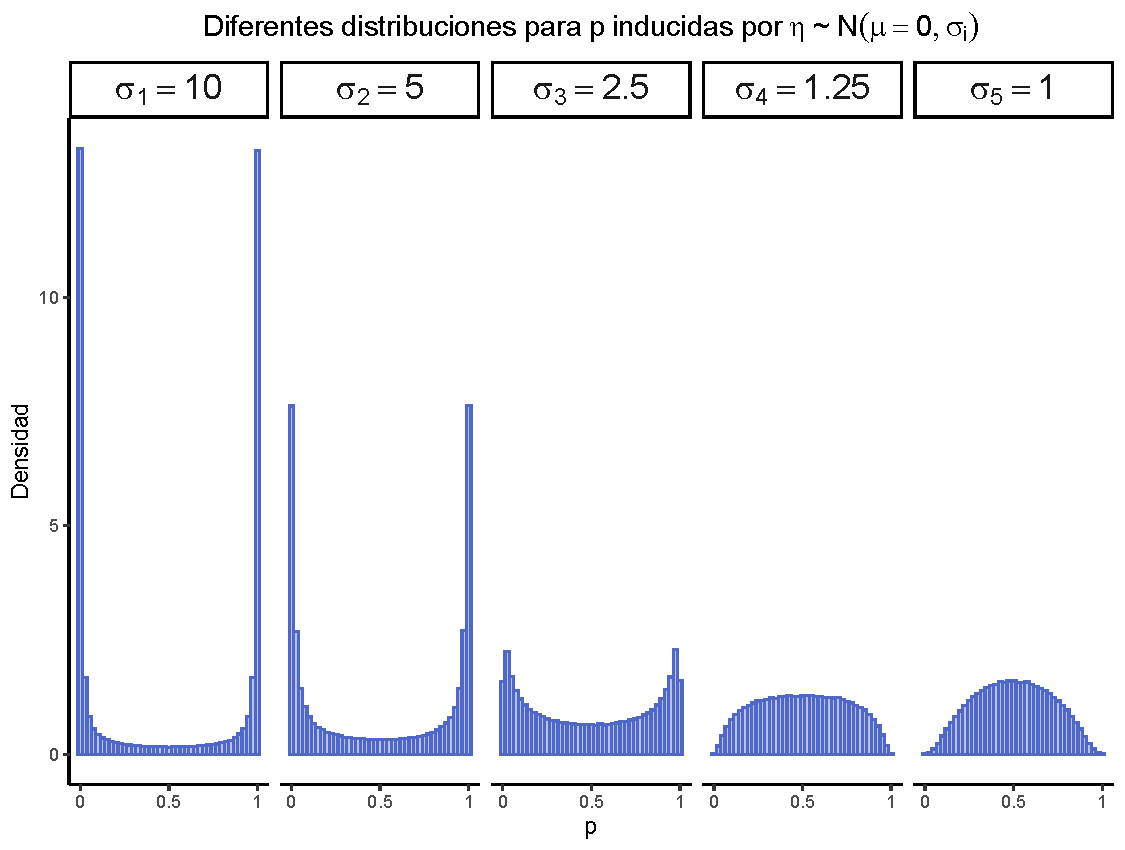
\includegraphics[width = 0.9\textwidth]{Figs/Modelado/Malas_Iniciales}
	\caption{Ejemplo de implicaciones en $p$ con distribuciones iniciales para un predictor lineal. Todas son normales centradas en $0$ con distintos parámetros $\sigma$ de desviación estándar. Fuente: elaboración propia.}
	\label{fig:Malas_Iniciales}
\end{figure}

El motivo es que la función logística no es lineal y tiene que ``compactar'' valores en los reales dentro del espacio confinado del $\left(0,1\right)$. Por decirlo de una manera informal, el verdadero rango de variación de la escala logística son valores de $\eta$ en $(-5,5)$; valores fuera de este intervalo llevan prácticamente a los mismos valores extremos cercanos a 0 o a 1, como apreciamos en la \textbf{Figura \ref{fig:Escala_Logis}}.\\

\begin{figure}[h]
	\centering
	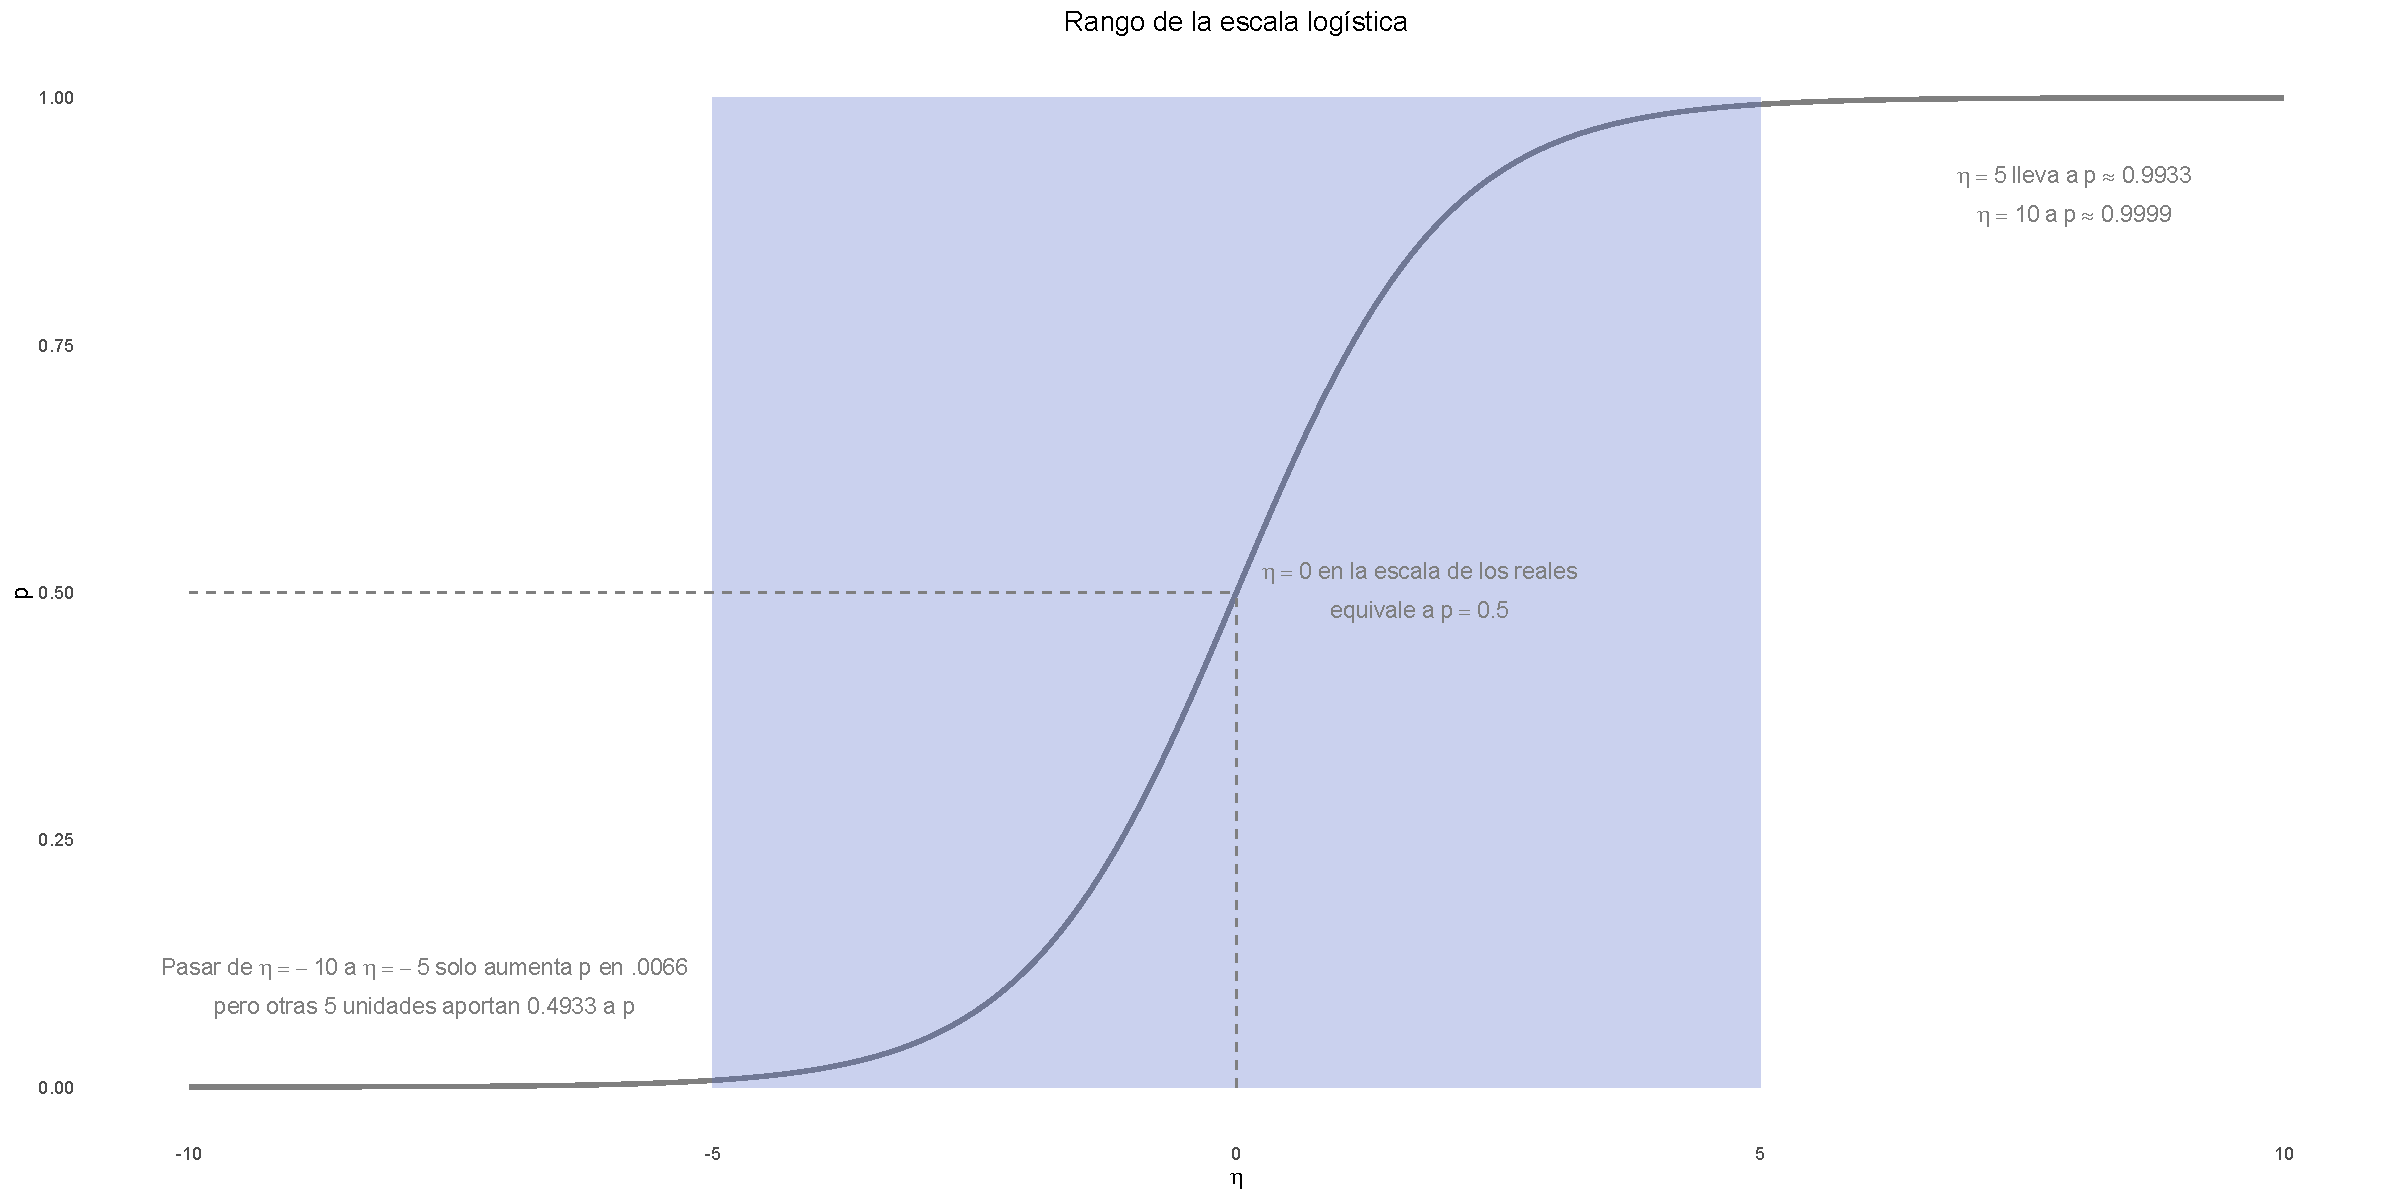
\includegraphics[width = 0.8\textwidth]{Figs/Modelado/Escala_Logis}
	\caption{Fuente: elaboración propia.}
	\label{fig:Escala_Logis}
\end{figure}

Ahora bien, nosotros no asignaremos distribuciones iniciales para el predictor lineal en su conjunto, sino para los coeficientes $\beta$ de dicho predictor lineal. Optaré aquí por una posición un poco escéptica o conservadora. A pesar de lo que sugerían las tendencias ingenuas del capítulo anterior, \textit{a priori}, no buscaría asignarle un sentido al efecto. Asimismo, los efectos de variables ecológicas o agregadas, no deberían ser tan grandes. No querría ``inflar'' la magnitud del valor explicativo mediante la distribución inicial pero tampoco negar la posibilidad de que existan algunos efectos importantes. Considero que una inicial para el coeficiente $\beta\sim N(\mu=0,\sigma=0.5)$ cumple relativamente bien con estas condiciones. Si tomamos el $0$ como referencia y comparamos el valor correspondiente de $p$ con aquel para una $\beta$ una desviación estándar mayor--- i.e. $\beta = 0.5$--- el efecto $\Delta$ sería de aproximadamente $+12$ puntos porcentuales. Si ahora disminuimos $\beta$ en 2 desviaciones estándar,  $\Delta \approx -23$ pp, como puede apreciarse en la \textbf{Figura \ref{fig:Inicial_Coef}}. Sin exagerar su interpretación, pues hay que multiplicar por el valor de la variable explicativa, estos podrían pensarse como los máximos efectos creíbles \textit{a priori}. 

\begin{figure}[h]
	\centering
	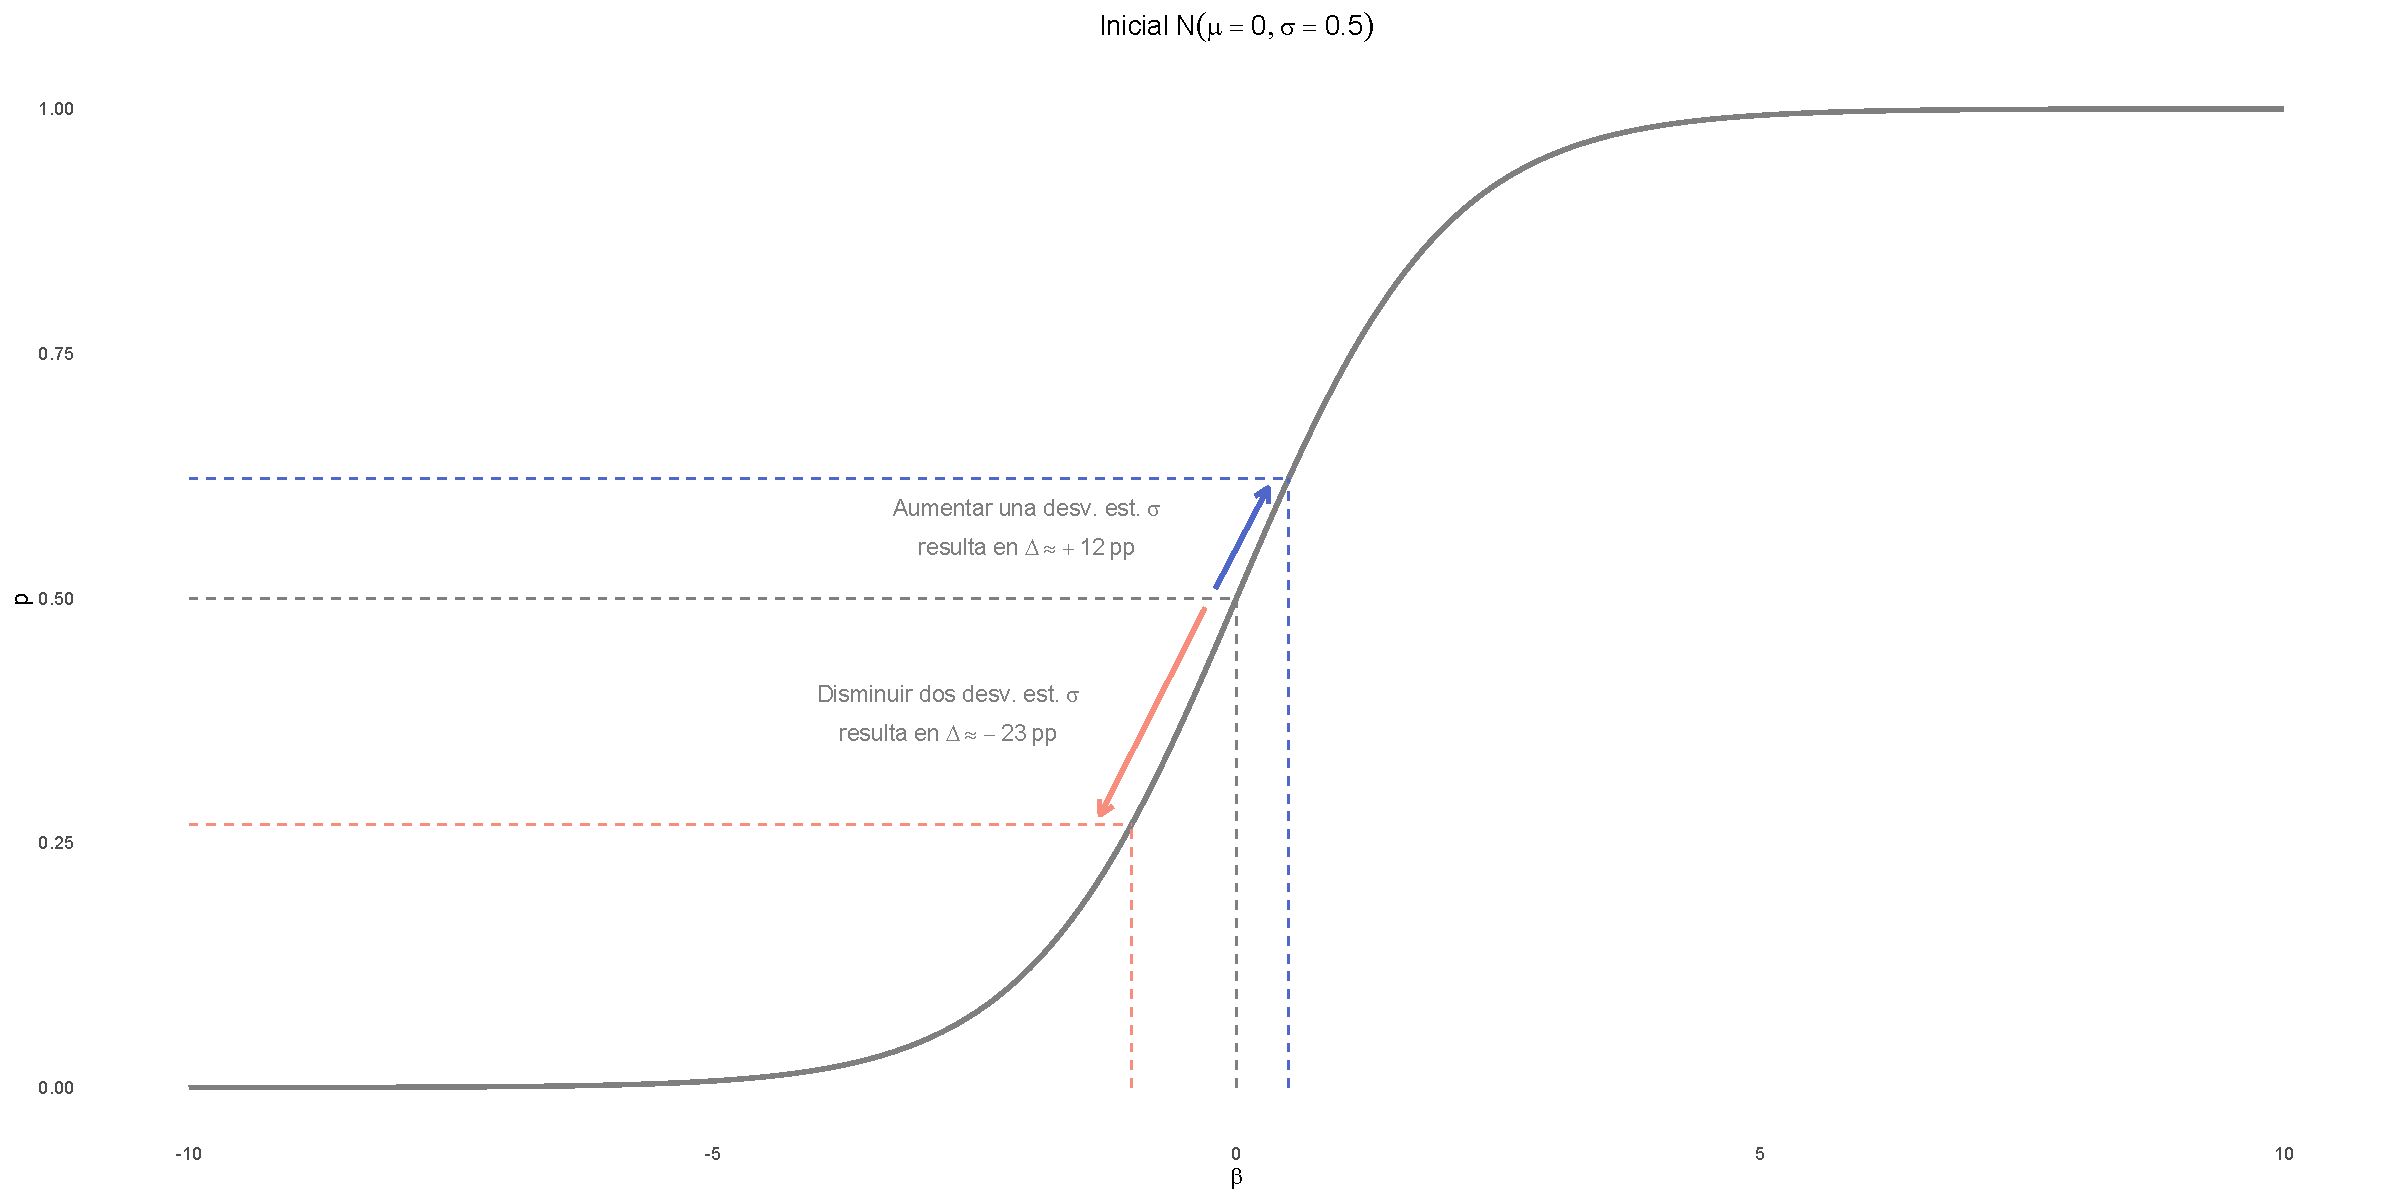
\includegraphics[width = 0.8\textwidth]{Figs/Modelado/Inicial_N0_un_medio}
	\caption{Fuente: elaboración propia.}
	\label{fig:Inicial_Coef}
\end{figure}

Por otro lado, debemos detenernos a pensar en la interpretación del intercepto $\alpha$. Por un lado, $\alpha$ es el valor que tomaría el predictor lineal $\eta_c$, si todos los coeficientes fueran iguales a $0$. Esto nos podría hacer pensar que querríamos que \textit{a priori} su distribución nos lleve a valores cercanos al  17.9\%, porcentaje que obtuvo Le Pen en la elección. Sin embargo, también hay que notar que con variables explicativas de configuraciones sociales, $x_c$, $\alpha$ es el valor que tomaría $\eta_c$ si la población estuviera repartida equitativamente entre todas las categorías. En efecto, supongamos que para la $m$-ésima variable con $l_m$ categorías cada $x_{j,c}=l_m^{-1}$. Tendríamos que

\begin{align*}
\eta_c &= \alpha + \sum\limits_{j=1}^{l_m} \beta_j x_{j,c} = \alpha + \sum\limits_{j=1}^{l_m} \dfrac{\beta_j}{l_m} = \alpha + \dfrac{1}{l_m}\sum\limits_{j=1}^{l_m} \beta_j
\intertext{y por la restricción de identificabilidad de suma cero de los coeficientes,}
&= \alpha + \dfrac{1}{l_m}\left(0\right) = \alpha 
\end{align*}

Tomando en cuenta las teorías del conflicto discutidas en la revisión de literatura, podríamos pensar que si en lugar de tener grupos mayoritarios frente a grupos minoritarios hubiese una sociedad más ``equilibrada'', el voto frontista disminuiría. Así pues, deberíamos buscar una distribución inicial con una media menor al 17.9\% obtenido en las elecciones. También, considerando que puede ser más robusto dilucidar una distribución inicial con base en cuantiles, más que igualar la media podríamos intentar aproximar el rango intercuartílico observado de entre 13.54\% y 21.44\%, pero sesgado un poco a la baja para tomar en cuenta la hipótesis anterior sobre una población equilibrada. Después de algunas pruebas elegí una distribución inicial para $\alpha\sim N(\mu = -1.7,\sigma = 0.25)$.\\

Consideremos ahora una ``comuna promedio'', definida como aquella que tuviera valores promedio en las variables explicativas; podemos realizar simulaciones de la distribución predictiva con estas iniciales. Es decir, simulamos de $\alpha\sim N(\mu = -1.7,\sigma = 0.25)$ y para cada $\beta\sim N(\mu = 0,\sigma = 0.5)$. Calculamos el predictor lineal con base en los valores promedio de cada categoría--- considerando también la restricción de suma cero de los coeficientes--- y tomamos el logit inverso. Este proceso, por ejemplo para grupos de edad, nos lleva al histograma de la \textbf{Figura \ref{fig:Predictiva_Inicial}}, con el modelo

\begin{align*}
y_c|\theta=(\alpha,\beta) & \sim Binom(n_c,p_c) \quad \forall \quad c \in \mathbb{N}_C \\
\text{con} \quad ln\left(\dfrac{p_c}{1-p_c}\right) &= \alpha + \beta_1Ed1_c + \dots + \beta_6Ed6_c \quad \text{tal que} \quad \beta_6 = -\sum\limits_{k = 1}^5 \beta_k \nonumber \\
\text{y} \quad \alpha & \sim N(\mu = -1.7,\sigma = 0.25)\\
\beta_j & \sim N(\mu = 0,\sigma = 0.5) \quad \, j =1,\dots,5
\end{align*}

\begin{figure}[h]
	\centering
	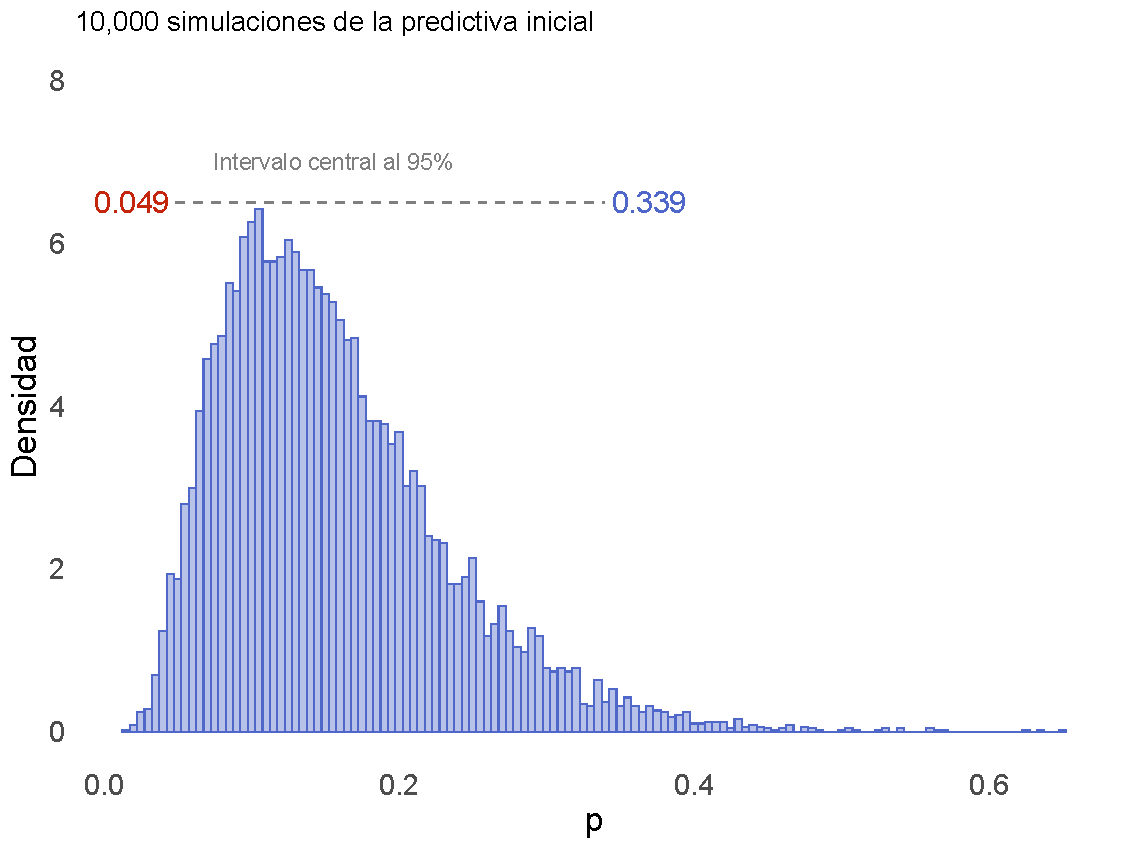
\includegraphics[width = 0.8\textwidth]{Figs/Modelado/Pred_Inicial}
	\caption{Fuente: elaboración propia.}
	\label{fig:Predictiva_Inicial}
\end{figure}

Estas distribuciones iniciales, como ya he mencionado, son subjetivas. Alguien más podría no estar muy convencido de la elección que realizo, por lo que eran importantes los párrafos anteriores de manera que fuera más transparente el proceso por el cual llegué a elegirlas.\\  

\section{Modelos individuales}

Consideremos entonces, para cada variable explicativa, modelos de la siguiente forma:

\begin{align}\label{eq:Modelo_Nal_Ind}
y_c|\theta=(\alpha,\beta) & \sim Binom(n_c,p_c) \quad \forall \quad c \in \mathbb{N}_C \nonumber \\
\text{con} \quad ln\left(\dfrac{p_c}{1-p_c}\right) &= \alpha + \sum\limits_{j=1}^{l_m} \beta_j x_{j,c} \quad \text{tal que} \quad \beta_{l_m} = -\sum\limits_{k = 1}^{l_m} \beta_k \nonumber \\
\text{y} \quad \alpha & \sim N(\mu = -1.7,\sigma = 0.25) \nonumber \\
\beta_j & \sim N(\mu = 0,\sigma = 0.5) \quad \, j \in \mathbb{N}_{l_m-1} 
\end{align}

A \eqref{eq:Modelo_Nal_Ind} le llamaré un \textbf{Modelo Nacional Individual} porque se tienen coeficientes a nivel nacional\footnote{En realidad, como mencionaba en el análisis exploratorio de datos, son coeficientes para la metrópoli y no para todo el país.} y solo incluyo una variable explicativa de manera individual. Tendría entonces 9 modelos nacionales individuales de esta forma. Sin embargo, el análisis exploratorio de datos sugería que se podría modelar de mejor manera dejando que los coeficientes e interceptos variasen para cada uno de los 96 departamentos. Es decir, podríamos construir igualmente 9 \textbf{Modelos Jerárquicos Individuales}. Si denotamos como $d[c]$ el \textit{departamento} al que pertenece la comuna $c$, el modelo jerárquico individual sería: 

\begin{align}\label{eq:Modelo_Jer_Ind}
y_c|\theta & \sim Binom(n_c,p_c) \quad \forall \, c \in \mathbb{N}_C \nonumber \\
\text{con} \quad ln\left(\dfrac{p_c}{1-p_c}\right) &= \alpha_{d[c]} + \sum\limits_{j=1}^{l_m} \beta_{d[c],j} x_{j,c} \nonumber\\ 
\text{tal que} \quad \beta_{d,l_m} &= -\sum\limits_{k = 1}^{l_m} \beta_{d,k} \nonumber \\
\alpha_d & \sim N(\mu_{\alpha}, \sigma=1) \quad \forall \, d \in \mathbb{N}_{96} \nonumber \\
\beta_{d,j} & \sim N(\mu_{\beta}, \sigma=1) \quad \forall \, j \in \mathbb{N}_{l_m-1}  \quad \text{y} \quad d \in \mathbb{N}_{96} \nonumber \\
\mu_{\alpha} &\sim N(-1.7,\sigma=0.25) \nonumber \\
\mu_{\beta} &\sim N(0,\sigma=0.5)
\end{align}

Se corrieron cada uno de los 18 modelos mediante el software Stan, simulando vía \textit{Hamiltonian Monte Carlo} las distribuciones posteriores dada la muestra de datos discutida en la \autoref{secc:muestra}. Una vez con dichas distribuciones posteriores, podemos hacer lo que \textcite{Gelman13} llaman \textit{posterior predictive checks}. Podemos predecir el porcentaje esperado de votos en cada una de las comunas y calcular su error respecto al real. Para el modelo nacional de ocupación laboral juvenil, los resultados están en la \textbf{Figura \ref{fig:Modelo_Nal_Ocu_Juvenil}}.\\

\begin{figure}[h]
	\centering
	\includegraphics[width = 0.8\textwidth]{Figs/Modelado/Modelo_Nal_Ocu_Juvenil}
	\caption{Mapa de predicciones medias del porcentaje bruto de votos obtenido por Marine Le Pen en las presidenciales 2012 mediante el Modelo Nacional por Ocupación Juvenil y mapa de los respectivos errores. Fuente: elaboración propia.}
	\label{fig:Modelo_Nal_Ocu_Juvenil}
\end{figure}

En el mapa de la izquierda las predicciones se colorean de acuerdo a la escala real que va de 0\% a 62.5\% y donde el cambio de tonos rojos a azules se da en la comuna mediana de 17.5\%. Observamos que la predicción en general subestima el verdadero porcentaje obtenido pues el mapa está prácticamente coloreado en su totalidad de tonos rojos. Sin embargo, las predicciones están cerca de la mediana. De hecho, el mapa de errores--- verde significa poco error y naranjas y rojos más--- visualmente es prácticamente un negativo del verdadero mapa de resultados que observábamos en la \textbf{Figura \ref{fig:Mapa_Pct_Br}} del capítulo anterior.\\

En general, los modelos nacionales tienen el defecto de no reconocer la enorme variabilidad geográfica del fenómeno electoral. Si construimos distintas medidas de error de predicción vemos que pasar de un modelado nacional a un modelado jerárquico las reduce consistentemente. Para cada simulación posterior predecimos el número de votos en cada comuna, departamento y a nivel nacional. Luego lo convertimos en porcentaje bruto de votos predicho dividiendo entre el número de inscritos en la comuna. Así, podemos tomar los conocidos errores absoluto y cuadrático promedio para el porcentaje de votos a nivel comuna, departamento y nacional. Incluso podemos tomar una pérdida más arbitraria, pero ilustrativa, como el porcentaje promedio de estimaciones que se encuentran a más de 1.5 puntos porcentuales del verdadero valor en los 3 niveles de agregación; a esta medida la llamo tolerancia 1.5 pp. Finalmente se calcula el promedio de las medidas a través del total de simulaciones posteriores y se grafican en la \textbf{Figura \ref{fig:Errores_Modelos_Individuales}}. El gráfico también incluye el cálculo de un cuarto error llamado WAIC para las comunas, pero a él me refiriré más adelante. En el gráfico, los puntos son las medidas para el modelo nacional y las flechas las de los modelos jerárquicos.\\ 

\begin{figure}[h]
	\centering
	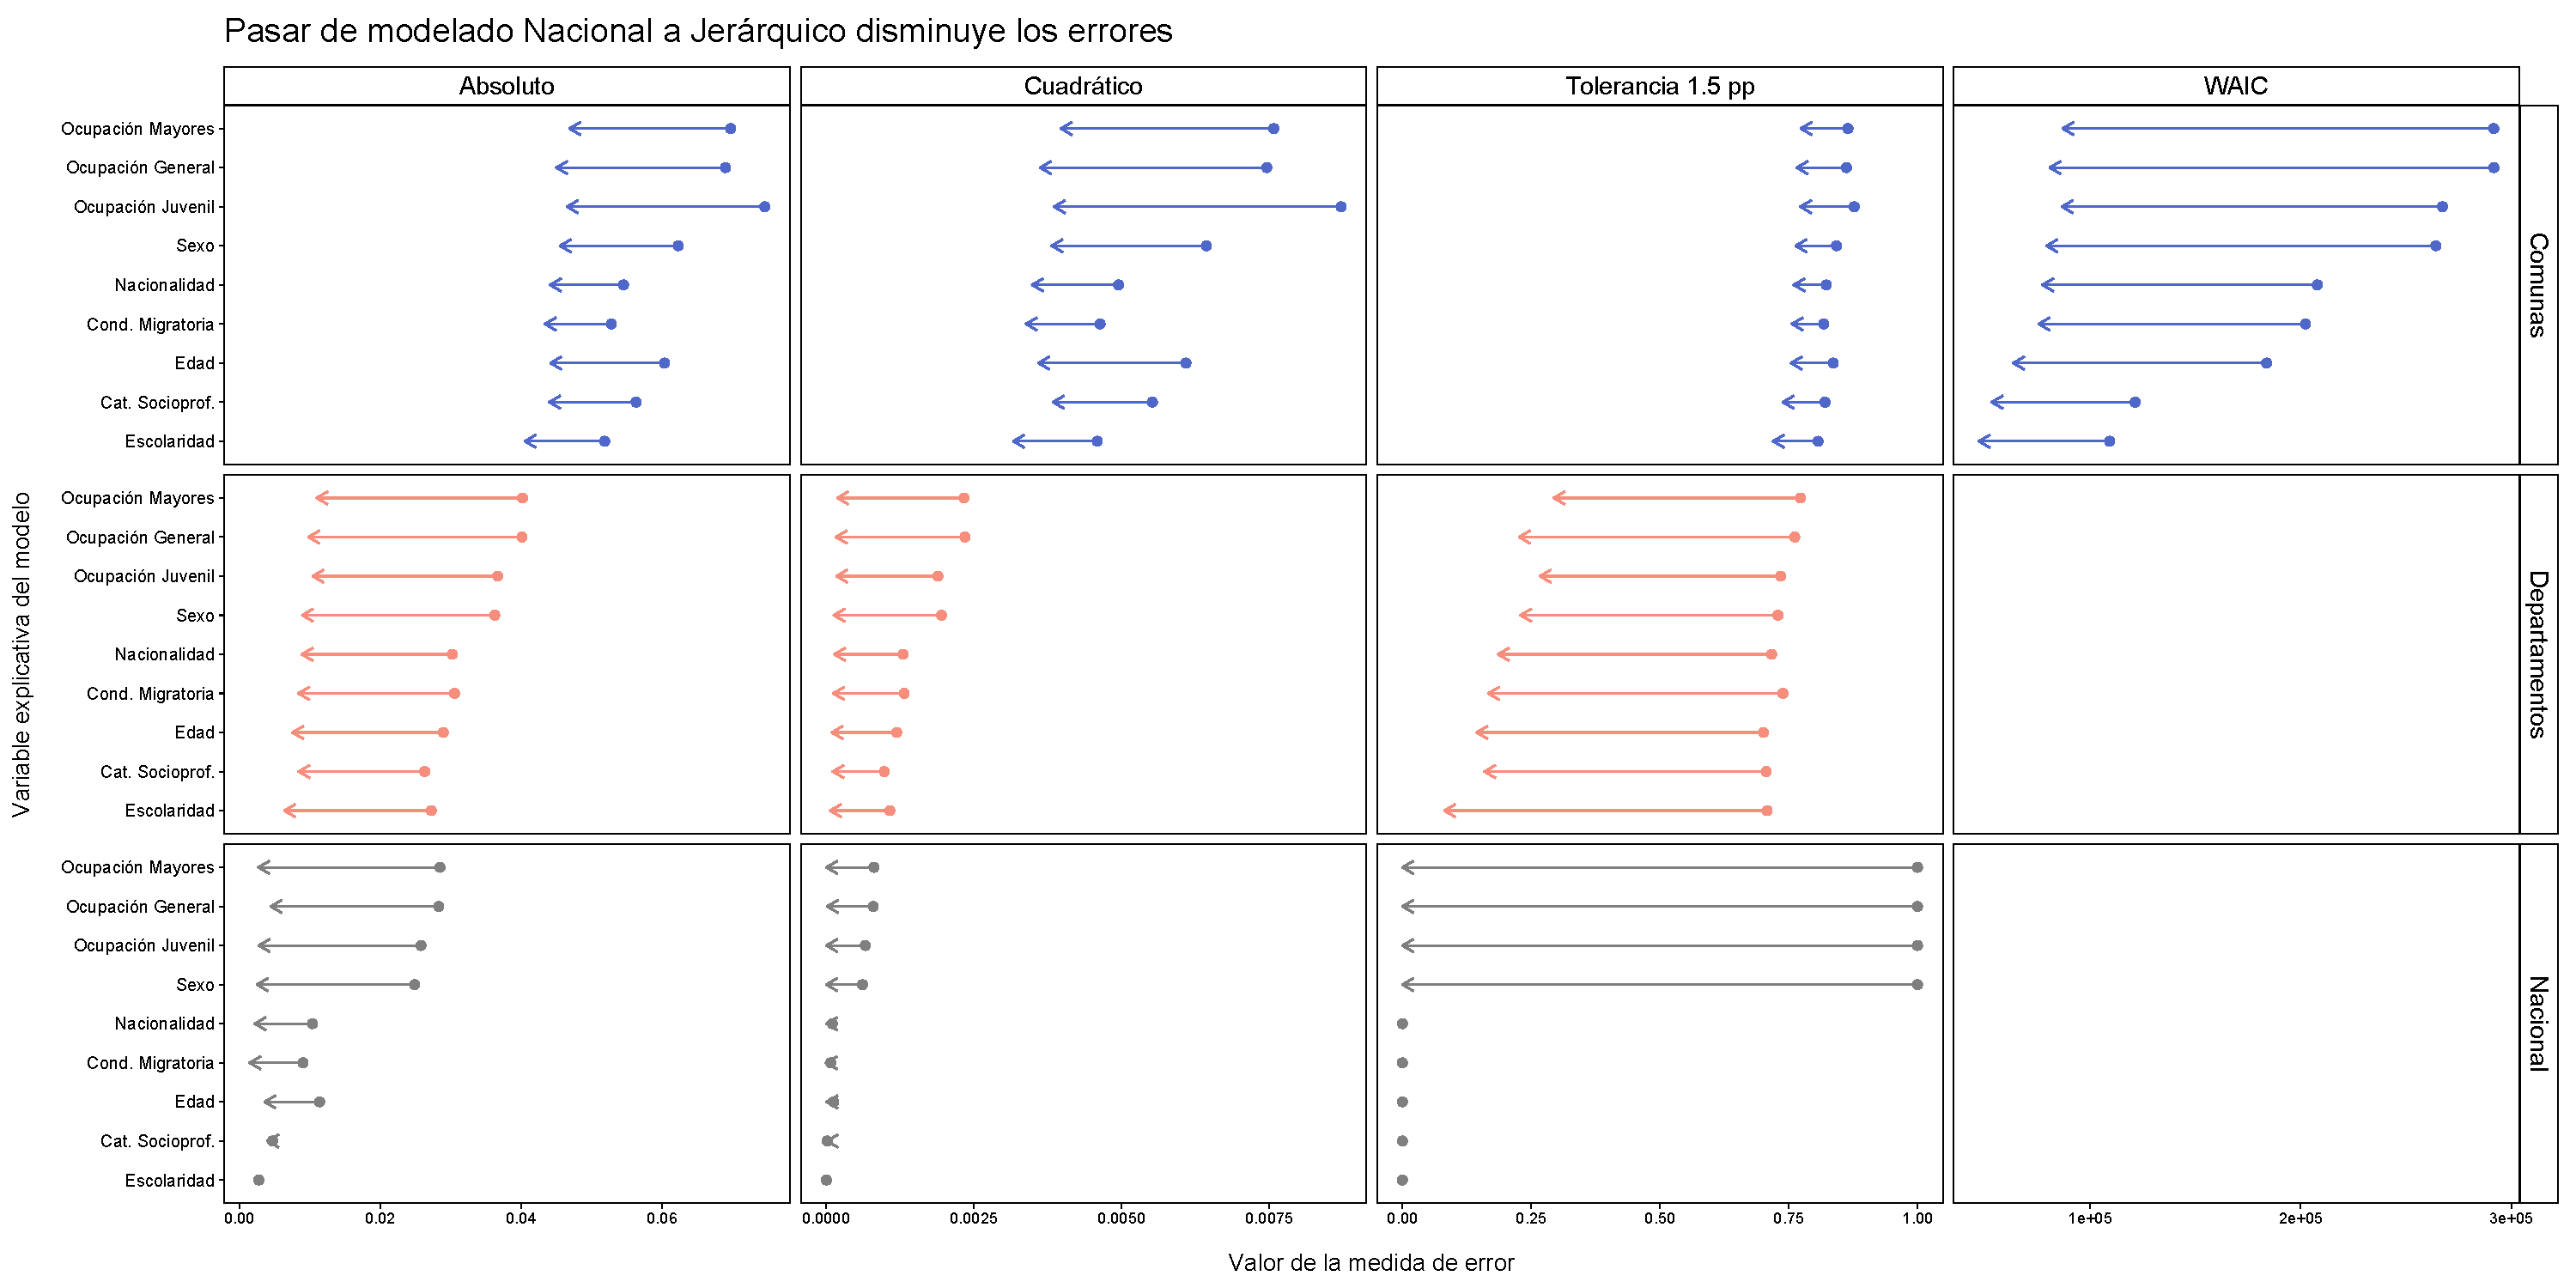
\includegraphics[width = 0.8\textwidth]{Figs/Modelado/Graf_Errores_Modelos_Individuales}
	\caption{Comparación de los modelos nacionales y jerárquicos individuales bajo diferentes medidas de error. Fuente: elaboración propia.}
	\label{fig:Errores_Modelos_Individuales}
\end{figure} 

Como es de esperarse, los modelos estiman de mejor manera los porcentajes de niveles de mayor agregación que el del nivel comunal. Viendo la pérdida arbitraria llamada de tolerancia 1.5, salvo las variables de sexo y ocupaciones, todas las predicciones estiman un porcentaje de votos nacional a menos de 1.5 puntos porcentuales del real. Sin embargo, vemos que para los 96 departamentos, los modelos nacionales solo logran esta precisión esperada de estimación en al rededor de 70. Esto refleja lo que había mencionado al ver el mapa de predicciones para el modelo nacional individual por ocupación juvenil. Al no permitir que los coeficientes varíen por departamento, el modelo ajusta para el país entero, sacrificando las estimaciones en las diferentes zonas geográficas que estos constituyen. Si observamos medidas de error más tradicionales como la absoluta o la cuadrática vemos que todas las flechas se dirigen a la izquierda, es decir que se reducen los errores al reconocer esa variabilidad geográfica. Ahora bien, estas 3 medidas tienen más un carácter ilustrativo y sirven para recordar que se pueden construir diferentes errores para diferentes estimadores.\\ 

Ahora notemos que las variables de solo 2 categorías como ocupación, sexo, nacionalidad y condición migratoria tienen peor desempeño que las de más categorías como edad, categoría socioprofesional y escolaridad. ¿Esto quiere decir que son peores variables explicativas? ¿No podría esto deberse a que las últimas tienen más parámetros y es más fácil ajustar mejor simplemente por introducir parámetros adicionales?\\

\subsection{WAIC}

Pensando en la posibilidad de mejorar un ajuste simplemente haciendo más complejo el modelo es que una mejor y más aceptada medida de error es el llamado WAIC por sus siglas en inglés \textit{Widely Applicable} o \textit{Watanabe-Akaike Information Criterion} \parencite{Vehtari16}. El WAIC busca estimar la capacidad predictiva de un modelo via las predictivas posteriores de los datos con los que se ajusta. La intuición es que a mayor valor de la predictiva posterior para el dato observado, mayor la posibilidad de predecir otros datos.\\ 

Para un conjunto de $n$ datos $y=(y_1,\dots,y_n)$ y una muestra posterior de parámetros $\left\lbrace\theta_{(s)}\right\rbrace_{s=1}^S$, el WAIC se define de la siguiente manera:

\begin{align}\label{WAIC}
WAIC(y|\theta) &= \widehat{lpd} + \widehat{par} \\
\text{con} \quad \widehat{lpd} &= \sum_{i=1}^{n} ln\left(\dfrac{1}{S}\sum\limits_{s=1}^S f(y_i|\theta_{(s)}) \right) \nonumber \\
\text{y} \quad \widehat{par} &= \sum\limits_{i=1}^n V(y_i|\theta), \nonumber
\end{align}

donde $V(y_i|\theta)=\dfrac{1}{S-1}\sum\limits_{s=1}^S \mathcal{L}(y_i;\theta_{s})^2$ y $\mathcal{L}(y_i;\theta_{s}) = ln\left[f(y_i|\theta_{(s)})\right] - \dfrac{1}{S}\sum\limits_{s=1}^S ln\left[f(y_i|\theta_{(s)})\right]$.{}\\

El WAIC se conforma de dos sumas. La primera, $\widehat{lpd}$, es una aproximación de la log predictiva posterior, es decir una medidad de ajuste. Por otro lado, $\widehat{par}$ es normalmente llamado el \textit{número efectivo estimado de parámetros} y es una medida que mediante sumas de varianzas busca medir la complejidad del modelo. En total, entre menor sea el valor del WAIC, esperaríamos un mejor desempeño predictivo tomando en cuenta la complejidad del modelo.\\ 

Notemos que con la definición dada, el WAIC es un estimador por lo que tiene una distribución muestral. Gracias al paquete \textit{loo} de $\mathsf{R}$, podemos estimar tanto los WAICs y sus errores estándar como la diferencia esperada entre dos de ellos y, {\color{Red} argumentando un teorema central del límite, la probabilidad de que el WAIC de un modelo sea efectivamente menor o igual al WAIC de otro. Estas comparaciones las observamos en la \textbf{Figura \ref{fig:Compara_WAIC_Individuales}}.}\\

\begin{figure}[h]
	\centering
	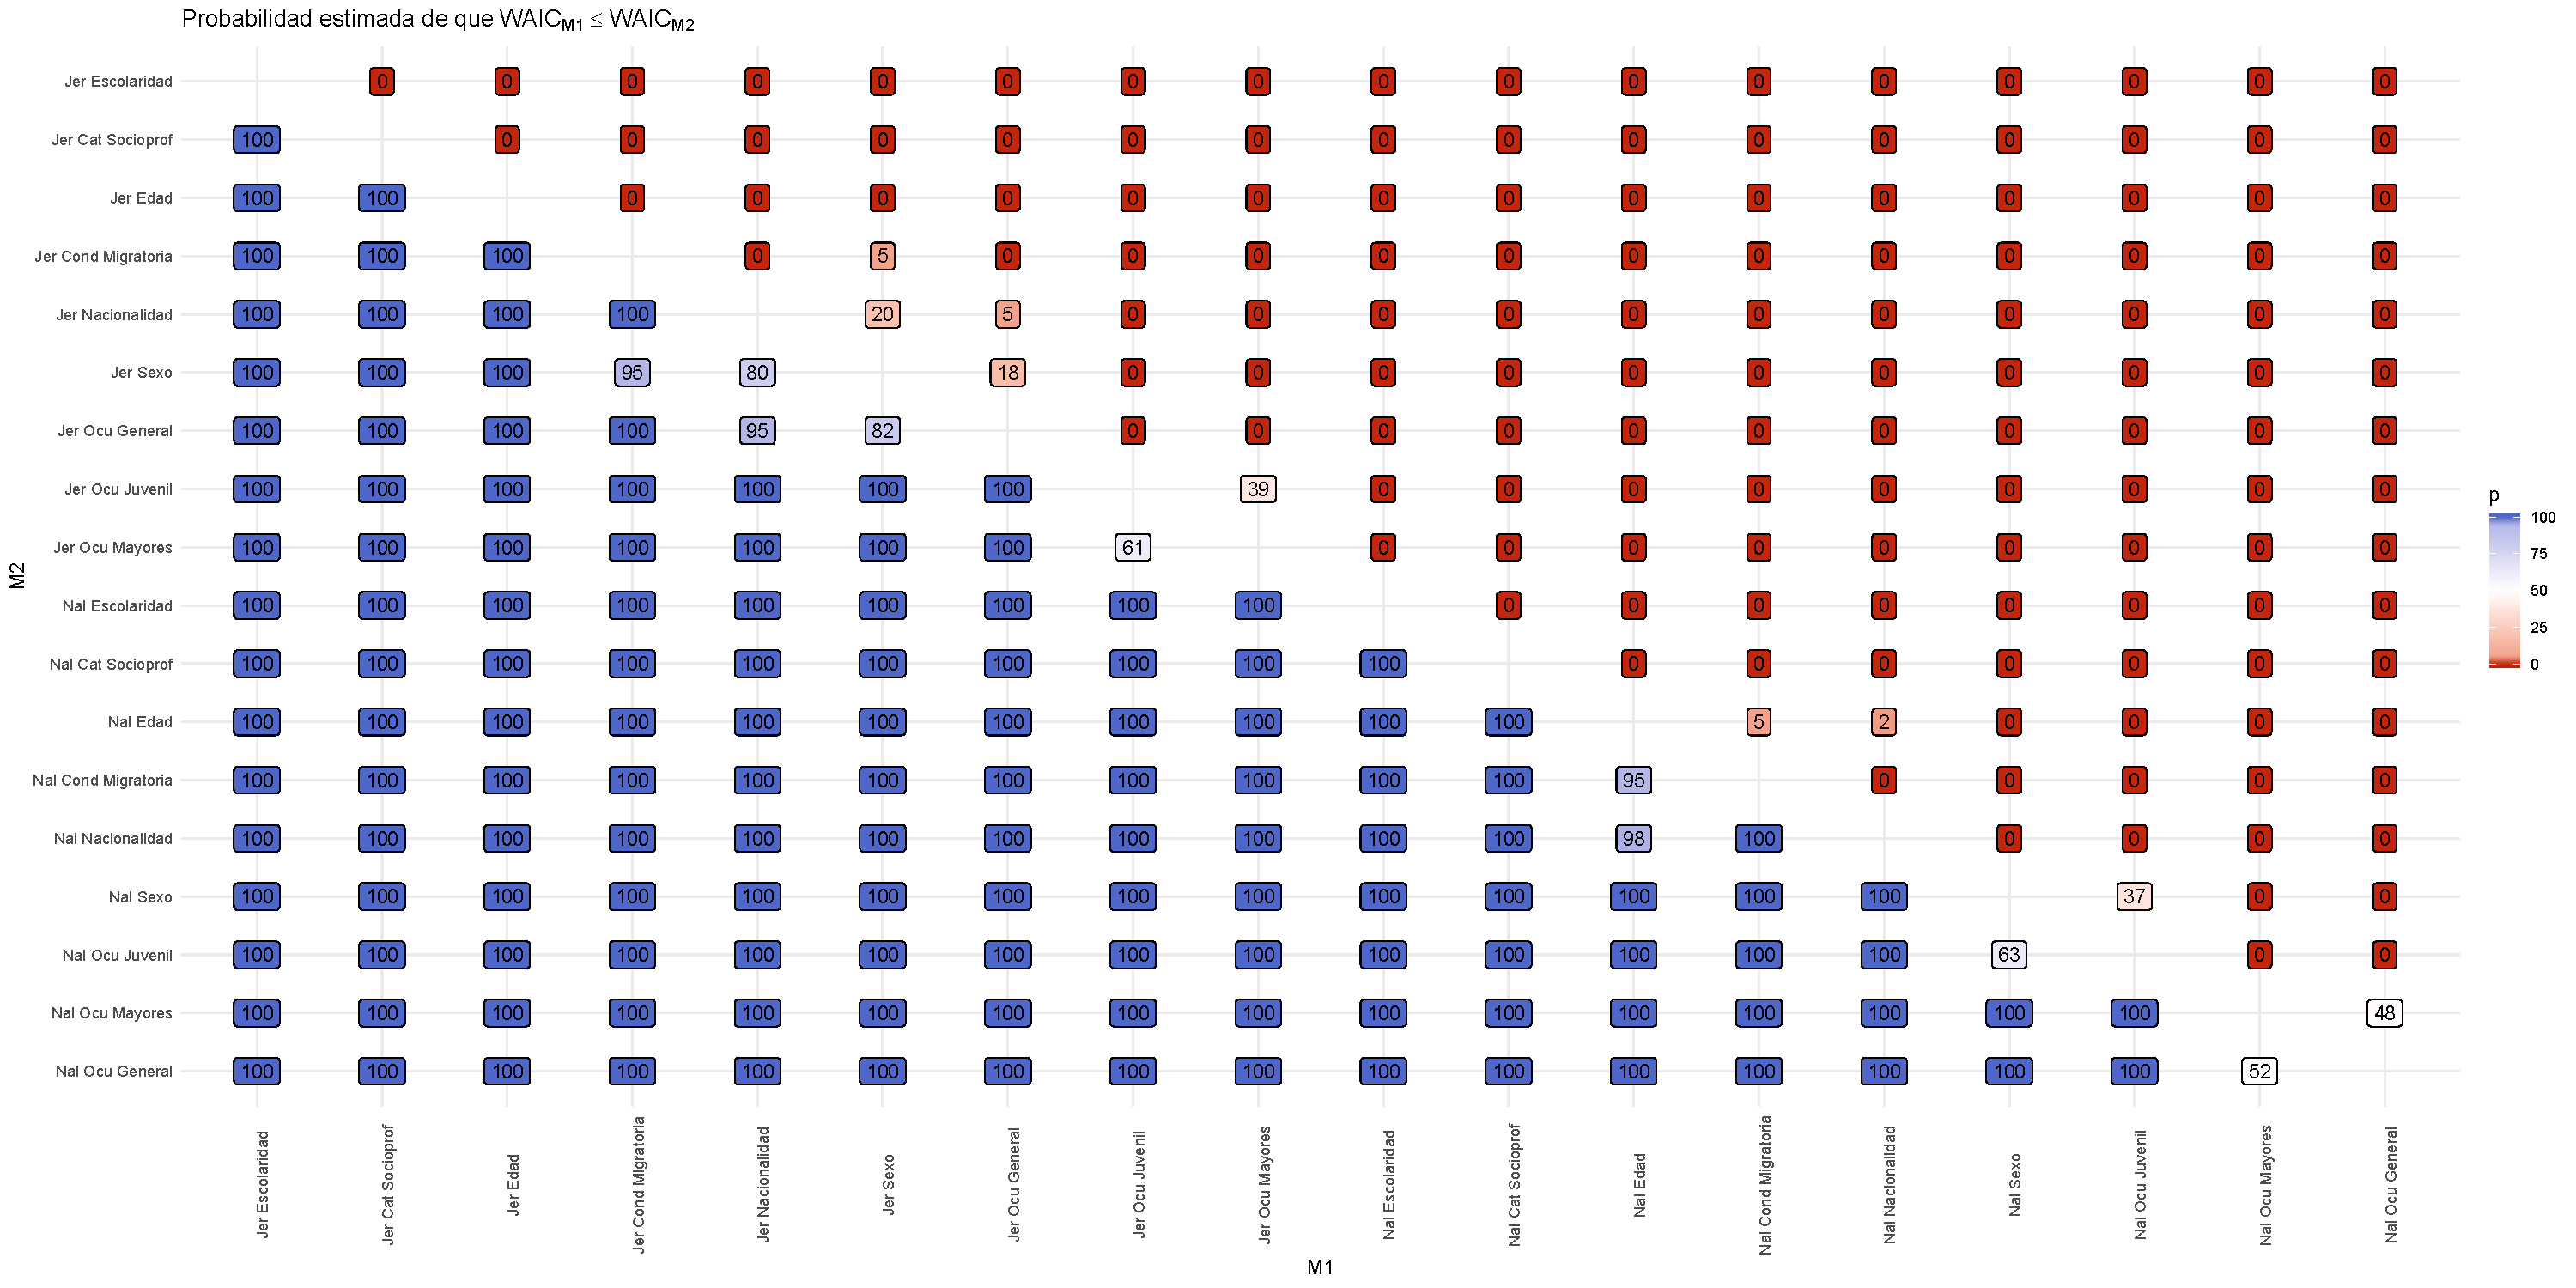
\includegraphics[width = 0.9\textwidth]{Figs/Modelado/Graf_WAIC_Probas_Modelos_Individuales}
	\caption{Comparativo de WAIC para distintos modelos. Fuente: elaboración propia con base en la estimación de la diferencia en WAIC proveniente de la función \textit{compare} del paquete \textit{loo} dentro $\mathsf{R}$ y asumiendo una distribución normal para la diferencia.}
	\label{fig:Compara_WAIC_Individuales}
\end{figure}

Para la mayoría de las comparaciones es claro que un modelo tiene mejor ajuste que el otro. Podríamos pensar que efectivamente hay un ordenamiento en el poder predictivo de las distintas variables: escolaridad, categorías socioprofesionales, edad, condición migratoria, nacionalidad, sexo y, finalmente, las ocupaciones. Sin concluir todavía nada, parecería que a las hipótesis sobre inseguridad laboral no les corresponde el mejor de los poderes explicativos en términos de estos modelos.\\

\section{Modelos Compuestos}

Este ordenamiento preliminar tiene el objetivo de ayudarme a construir, secuencialmente, un modelo cada vez más complejo. Para comenzar, veamos los mapas de predicción que generó el modelo con menor WAIC, el jerárquico por escolaridad, en la \textbf{Figura \ref{fig:Modelo_Jer_Escolaridad}}.\\ 

\begin{figure}[h]
	\centering
	\includegraphics[width = 0.8\textwidth]{Figs/Modelado/Modelo_Jer_Escolaridad}
	\caption{Mapa de predicciones medias del porcentaje bruto de votos obtenido por Marine Le Pen en las presidenciales 2012 mediante el Modelo Jerárquico por Escolaridad y mapa de los respectivos errores. Fuente: elaboración propia.}
	\label{fig:Modelo_Jer_Escolaridad}
\end{figure}

El mapa de errores ya se observa más verde y homogéneo. Las grandes zonas de fortaleza y debilidad del FN comienzan a ser identificadas por el modelo. Sin embargo, los tonos de algunas predicciones son todavía demasiado cercanos a la mediana. En el centro observamos una zona de tonos muy claros, casi blancos, que no corresponden totalmente a la realidad. En general, vemos que hay menor variabilidad dentro de los departamentos de la que se observó en la elección.\\ 

Estas reflexiones sugieren que, en lugar de tomar una a una las variables, podemos ir agregando variables a la regresión en modelos jerárquicos secuenciales que refinen el ajuste. Entonces, este modelo jerárquico por escolaridad podríamos considerarlo el \textbf{Modelo 0}, pues partiremos de él para ir agrandándolo con la inclusión de una nueva variable cada vez.\\ 

El primer modelo compuesto incluye las variables de escolaridad y categorías socioprofesionales. A este modelo lo llamaré el \textbf{Modelo A}. Para distinguir las variables utilizaré diferentes letras griegas para sus coeficientes. Para la configuración social de escolaridad 
\[x_{escol,c} = (Esc_c,Dip1_c,Dip2_c,Dip3_c,Dip4_c)^T\]
en la comuna $c$ los coeficientes departamentales serán un vector $\beta_{d[c]} = (\beta_{d[c],1},\dots,\beta_{d[c],5})$. Para las categorías socioprofesionales $x_{csp,c}$ los coeficientes serán $\gamma_{d[c]}$:

\begin{align}\label{eq:Modelo_Comp_A}
y_c|\theta & \sim Binom(n_c,p_c) \quad \forall \, c \in \mathbb{N}_C \nonumber \\
\text{con} \quad ln\left(\dfrac{p_c}{1-p_c}\right) &= \alpha_{d[c]} + \beta_{d[c]} x_{escol,c} + \gamma_{d[c]} x_{csp,c} \\ 
\intertext{tal que} 
\beta_{d,5} &= -\sum\limits_{k = 1}^{4} \beta_{d,k}, \nonumber \\
\gamma_{d,8} &= -\sum\limits_{k = 1}^{7} \gamma_{d,k} \nonumber \\
\intertext{donde $\forall \, d \in \mathbb{N}_{96}$}
\alpha_d & \sim N(\mu_{\alpha}, \sigma=1) \quad  \nonumber \\
\beta_{d,j} & \sim N(\mu_{\beta}, \sigma=1) \quad \forall \, j \in \mathbb{N}_{4} \nonumber \\
\gamma_{d,j} & \sim N(\mu_{\gamma}, \sigma=1) \quad \forall \, j \in \mathbb{N}_{7} \nonumber \\
\intertext{y}
\mu_{\alpha} &\sim N(-1.7,\sigma=0.25) \nonumber \\
\mu_{\beta} &\sim N(0,\sigma=0.5) \nonumber \\
\mu_{\gamma} &\sim N(0,\sigma=0.5) \nonumber
\end{align}

Al estimar el modelo con ambas variables las predicciones efectivamente mejoran. La diferencia en WAIC entre el modelo A y el modelo jerárquico por escolaridad se estima en -1594.7 con un error estándar de 175.2. Asimismo, observando los mapas de la \textbf{Figura \ref{fig:Modelo_Compuesto_A}}, vemos que se reduce la gran zona blanquiza del centro, se comienza a observar mayor variabilidad dentro de los departamentos y los tonos también se oscurecen más, sobre todo en el noreste.\\ 

\begin{figure}[h]
	\centering
	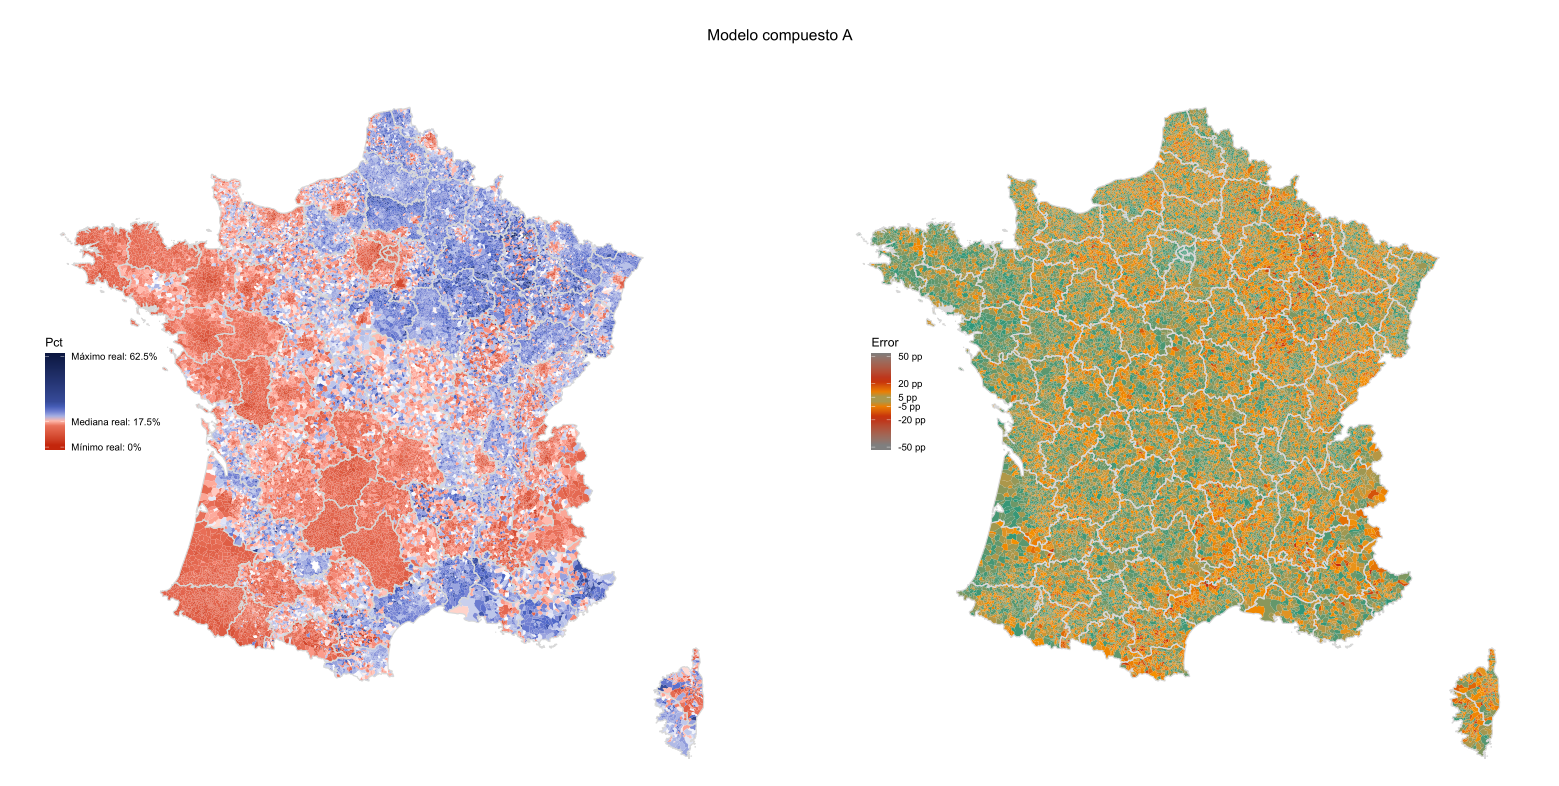
\includegraphics[width = 0.8\textwidth]{Figs/Modelado/Modelo_Compuesto_A}
	\caption{Mapas de predicciones medias y respectivos errores para el porcentaje bruto de votos obtenido por Marine Le Pen en las presidenciales 2012 mediante el Modelo Jerárquico por Escolaridad y Categorías socioprofesionales. Fuente: elaboración propia.}
	\label{fig:Modelo_Compuesto_A}
\end{figure}


Los siguientes modelos se llamarán de manera progresiva por letras latinas y sus planteamientos en términos de ecuaciones pueden encontrarse en el \autoref{Anexo_modelos_compuestos}. Por ejemplo, el \textbf{Modelo B} incorpora los grupos de edad $x_{edad,c}$. Al hacerlo, el WAIC vuelve a disminuir, ahora 965.4 unidades, y los respectivos mapas corresponden a la \textbf{Figura \ref{fig:Modelo_Compuesto_B}}.\\ 

\begin{figure}[h]
	\centering
	\includegraphics[width = 0.8\textwidth]{Figs/Modelado/Modelo_Compuesto_B}
	\caption{Mapas de predicciones medias y respectivos errores para el porcentaje bruto de votos obtenido por Marine Le Pen en las presidenciales 2012 mediante el Modelo Jerárquico por Escolaridad, Categorías socioprofesionales y Edad. Fuente: elaboración propia.}
	\label{fig:Modelo_Compuesto_B}
\end{figure}

Debido a la similitud entre condición migratoria y nacionalidad, solamente buscaba incorporar una de las dos, tratando de identificar la que tuviera mejor desempeño. De acuerdo al ordenamiento previo en los modelos individuales, consideraré solo la variable migratoria $x_{migr,c}$ dentro del \textbf{Modelo C}. Por su parte, el \textbf{Modelo D} incluye la distribución comunal por sexo $x_{sexo,c}$. {\color{Red} No presento los mapas por brevedad, pero de necesitarse se incluyen pues ya están generados}.\\

Después comenzaríamos a incluir las variables de ocupación. Como mencionaba al presentarlas, tengo un interés especial en la (des)ocupación juvenil, pues esta sería una variable que referencias como \textcite{LeBras16} y \textcite{Perrineau07} favorecerían. Por ello, al margen del ordenamiento, construí dos modelos de 6 variables. De manera general ambos incorporan una variable explicativa $x_{ocu,c}$. El \textbf{Modelo E} es el modelo D más la ocupación juvenil, mientras que el \textbf{Modelo F} es el modelo D más la ocupación general. Una vez generados por separado, podemos considerar un modelo que incorpre ambas variables, este sería el \textbf{Modelo G}. Finalmente agregamos la última variable considerada, la ocupación para personas de 55 a 64 años $x_{ocu\_may,c}$, para obtener el \textbf{Modelo H}.\\

¿Cuál es la comparación de WAICs entre ellos? En la \textbf{Figura \ref{fig:Compara_WAIC_Compuestos}} podemos observarlo. En general, el WAIC mejora conforme se van agregando variables. Ciertamente las mayores ganancias se dan al agregar las primeras variables que el análisis individual sugería eran las más explicativas. Esto parece confirmar dicha hipótesis. Por el contrario, en términos de WAIC, la ocupación juvenil no parece ser la más poderosa de las variables. En efecto, la ganancia en WAIC frente al modelo D al agregarla en el modelo E es de apenas 46 unidades, menor a la ganancia del modelo F que fue de 162. Más aún, al pasar del modelo F al modelo G agregándola de nuevo, la ganancia vuelve a ser poca, apenas de 29. Esto no quiere decir, sin embargo, que no aporte nada a la regresión. Aunque la mejora en WAIC sea pequeña y los intervalos con error estándar se traslapen, {\color{Red} la probabilidad de que agregarla produce un mejor modelo es de 84\% en el caso del modelo E y de 77\% en el modelo G.}

\begin{figure}[h]
	\centering
	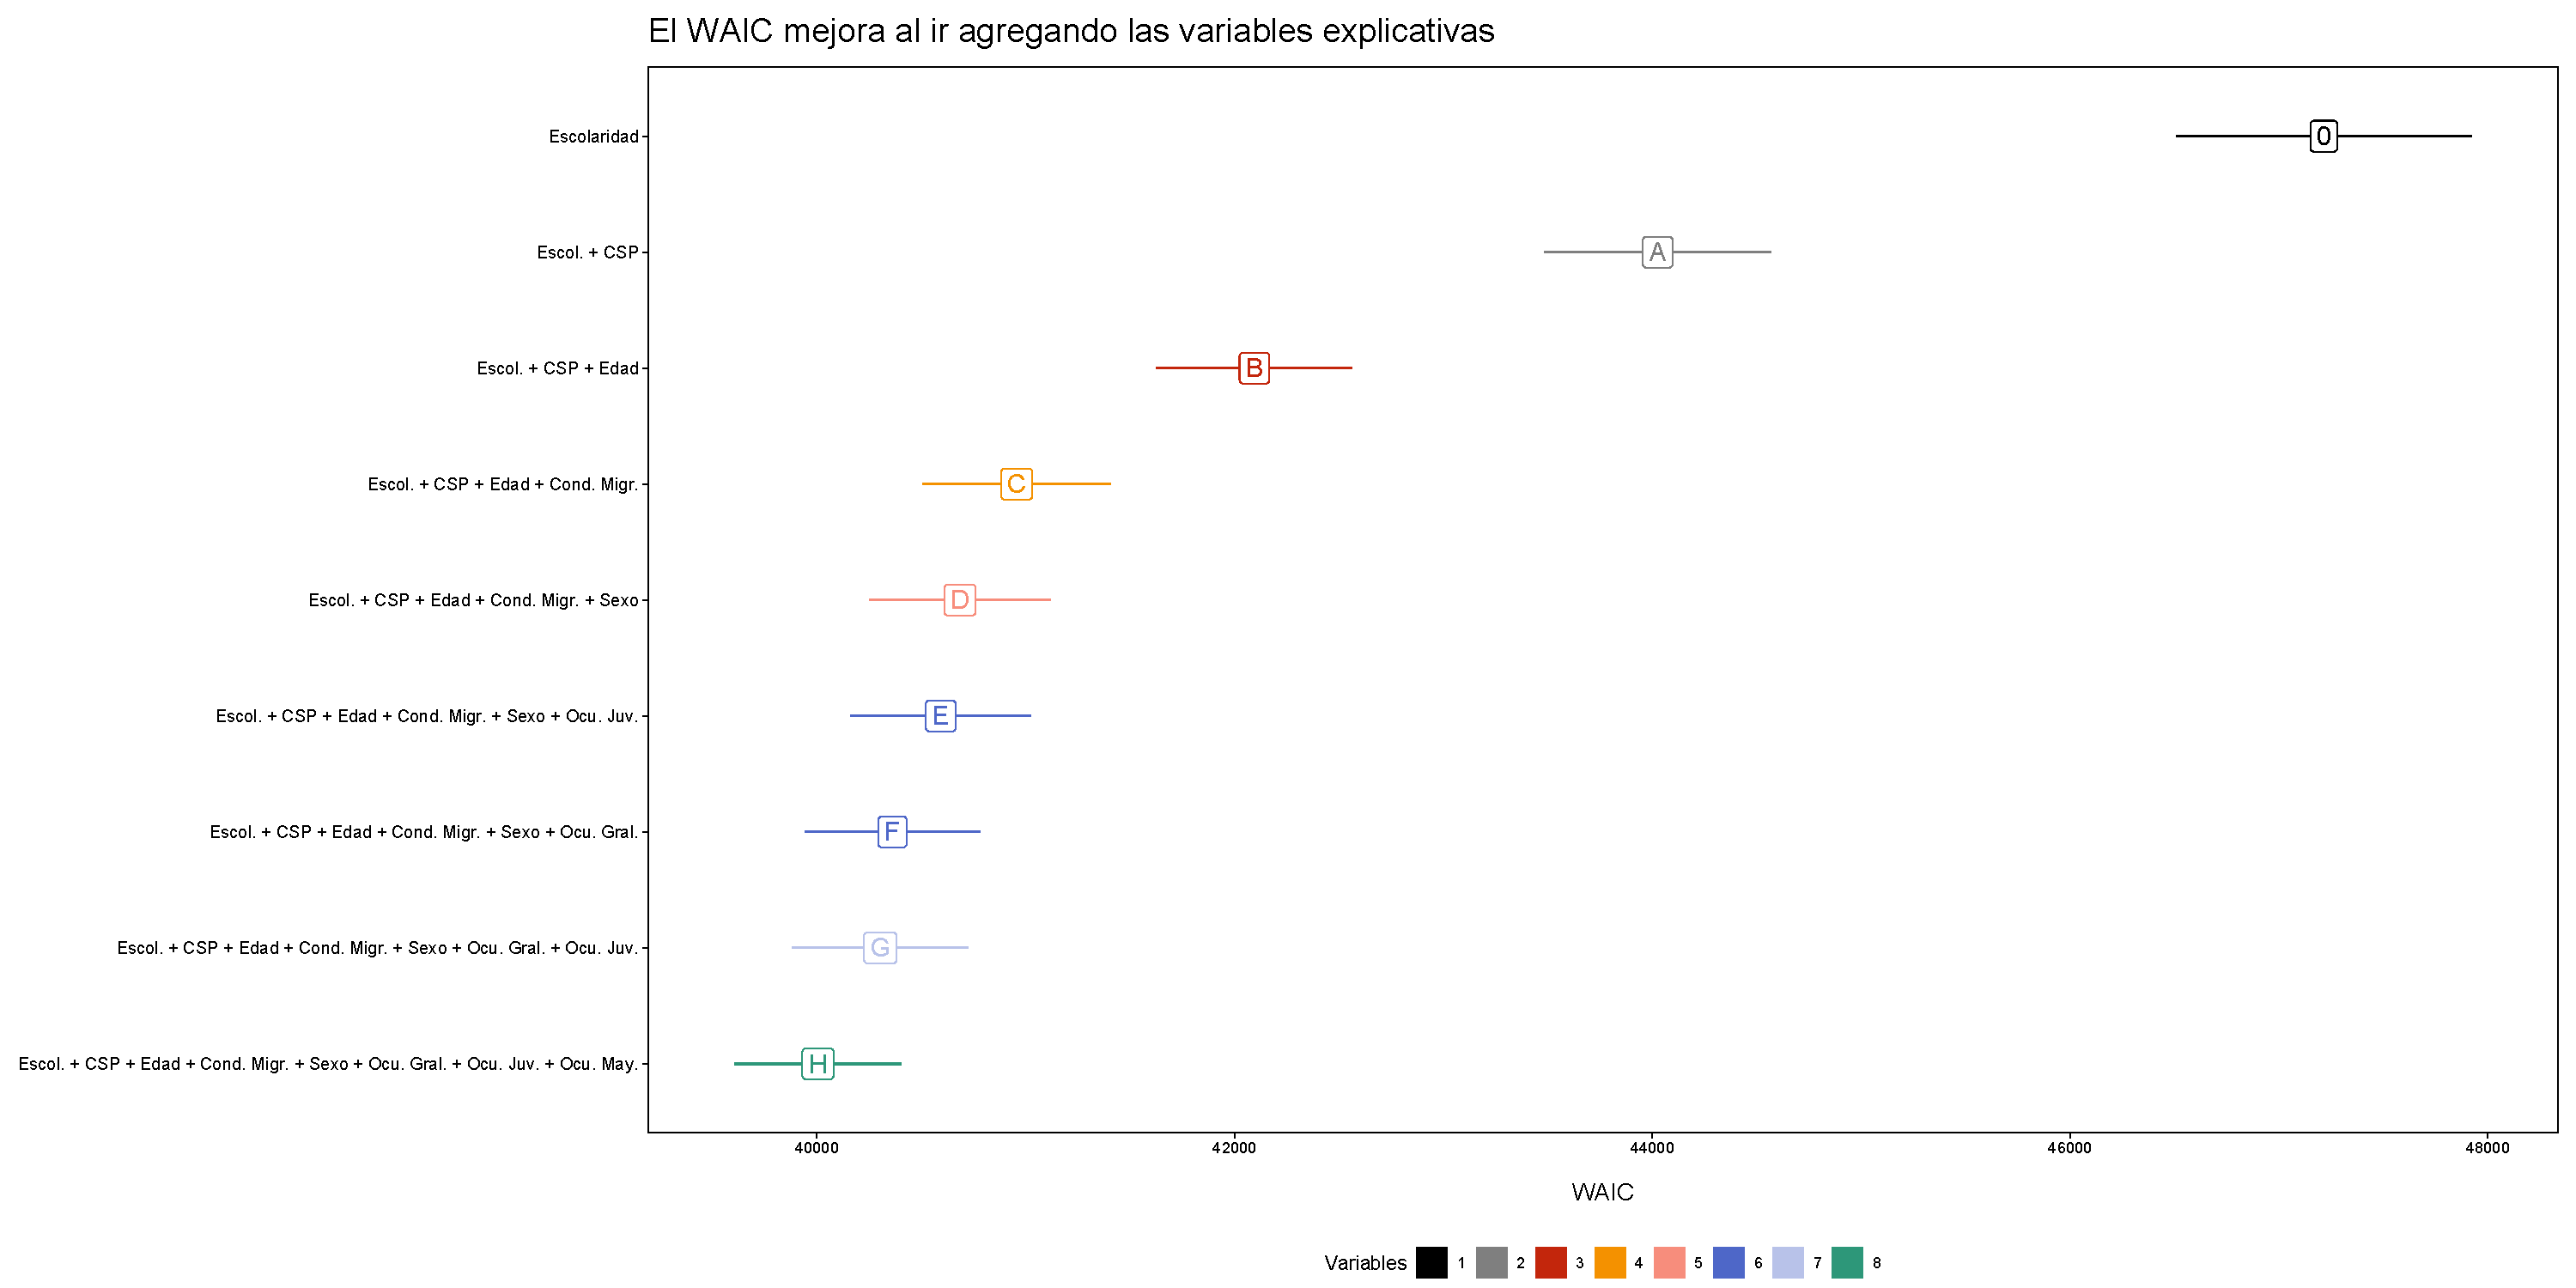
\includegraphics[width = 0.9\textwidth]{Figs/Modelado/Graf_WAIC_Modelos_Compuestos}
	\caption{Comparativo de WAIC para distintos modelos. Comenzando por el modelo 0 que incluye solo escolaridad se van añadiendo variables hasta incluirlas todas en el modelo H. Fuente: elaboración propia.}
	\label{fig:Compara_WAIC_Compuestos}
\end{figure}

\subsection{Convergencia de HMC}

Una vez ajustados los modelos, como adelantaba en la \autoref{sec:Convergencia}, habría que verificar que las cadenas simuladas mediante la implementación de HMC dentro de Stan hubieran convergido. Debido a la cantidad de parámetros dentro de cada modelo, así como a la cantidad de modelos ajustados en sí, es difícil verificar a detalle todas y cada una de las muestras posteriores. Afortunadamente, \textcite{BetancourtRStanWorkflow} desarrolla un caso de estudio en el que ilustra cómo realizar distintos diagnósticos útiles para todos los parámetros de interés dentro de todos los modelos. Entre ellos encontramos el factor de reducción de escala $\hat{R}$, así como un cálculo del tamaño efectivo de muestra por iteración y 3 diagnósticos particulares de HMC. Utilizando su código abierto\footnote{Los derechos de autor son de Michael Betancourt y la Universidad de Columbia y las licencias pueden verificarse en el link en las referencias.}, verificamos que los modelos satisfacen los criterios planteados y podemos confiar en la convergencia de las muestras posteriores obtenidas. {\color{Red} Esta comprobación puede reproducirse con el código del repositorio de Github de esta tesis y solicitándome acceso a los archivos .rds con los ajustes de todos los modelos.}\\

 Adicionalmente, podemos observar algunos diagnósticos gráficos para algunos parámetros del modelo H. Por ejemplo, en la \textbf{Figura \ref{fig:Traceplots_H}} observamos en los \textit{traceplots} para algunos parámetros que hay una buena mezcla de las cadenas; esto también se confirma viendo que las densidades por cadena de la \textbf{Figura \ref{fig:Densidades_H}} son parecidas. Finalmente, en la \textbf{Figura \ref{fig:Autocorr_H}} vemos que las autocorrelaciones son pequeñas. De hecho, existe un poco de simulación antitética que permite una mejor eficiencia en el tamaño de muestra \parencite{BlogAntithetical}.\\ 
 
 \begin{figure}[h]
	\centering
	\begin{subfigure}{0.45\textwidth}
	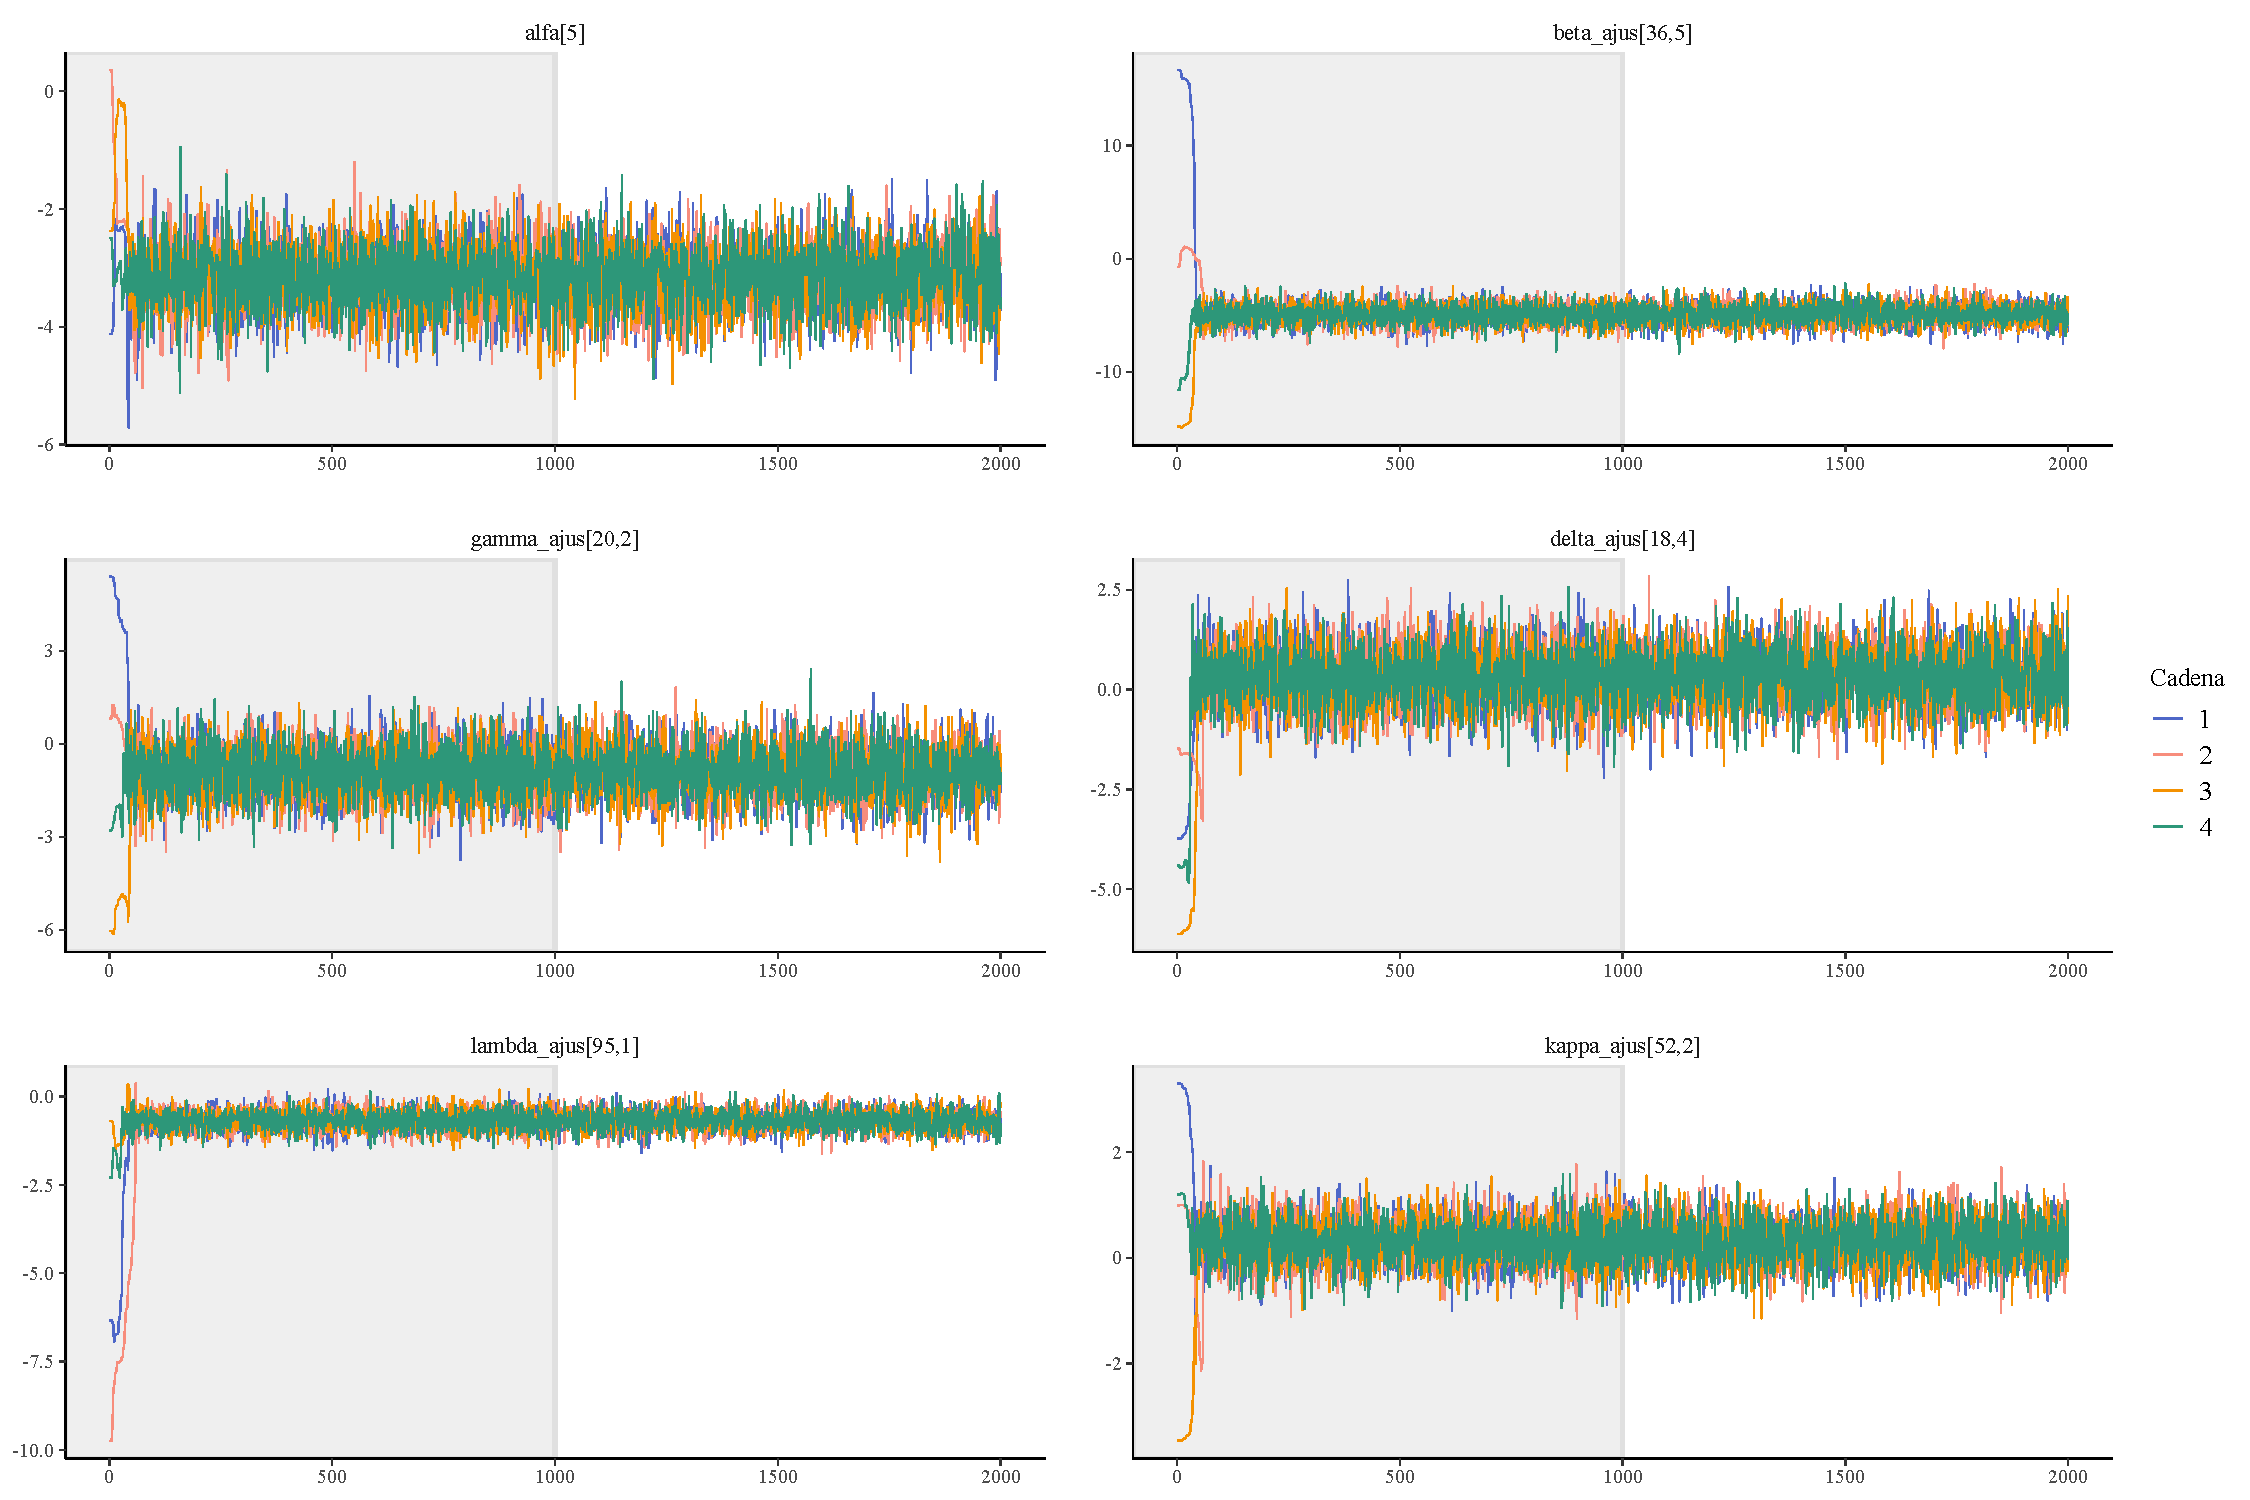
\includegraphics[width = \textwidth]{Figs/Convergencia/Convergencia_Traceplots}
	\caption{Ejemplo de \textit{traceplots} para algunos parámetros del modelo H.}
	\label{fig:Traceplots_H}
	\end{subfigure}
	~
	\begin{subfigure}{0.45\textwidth}
	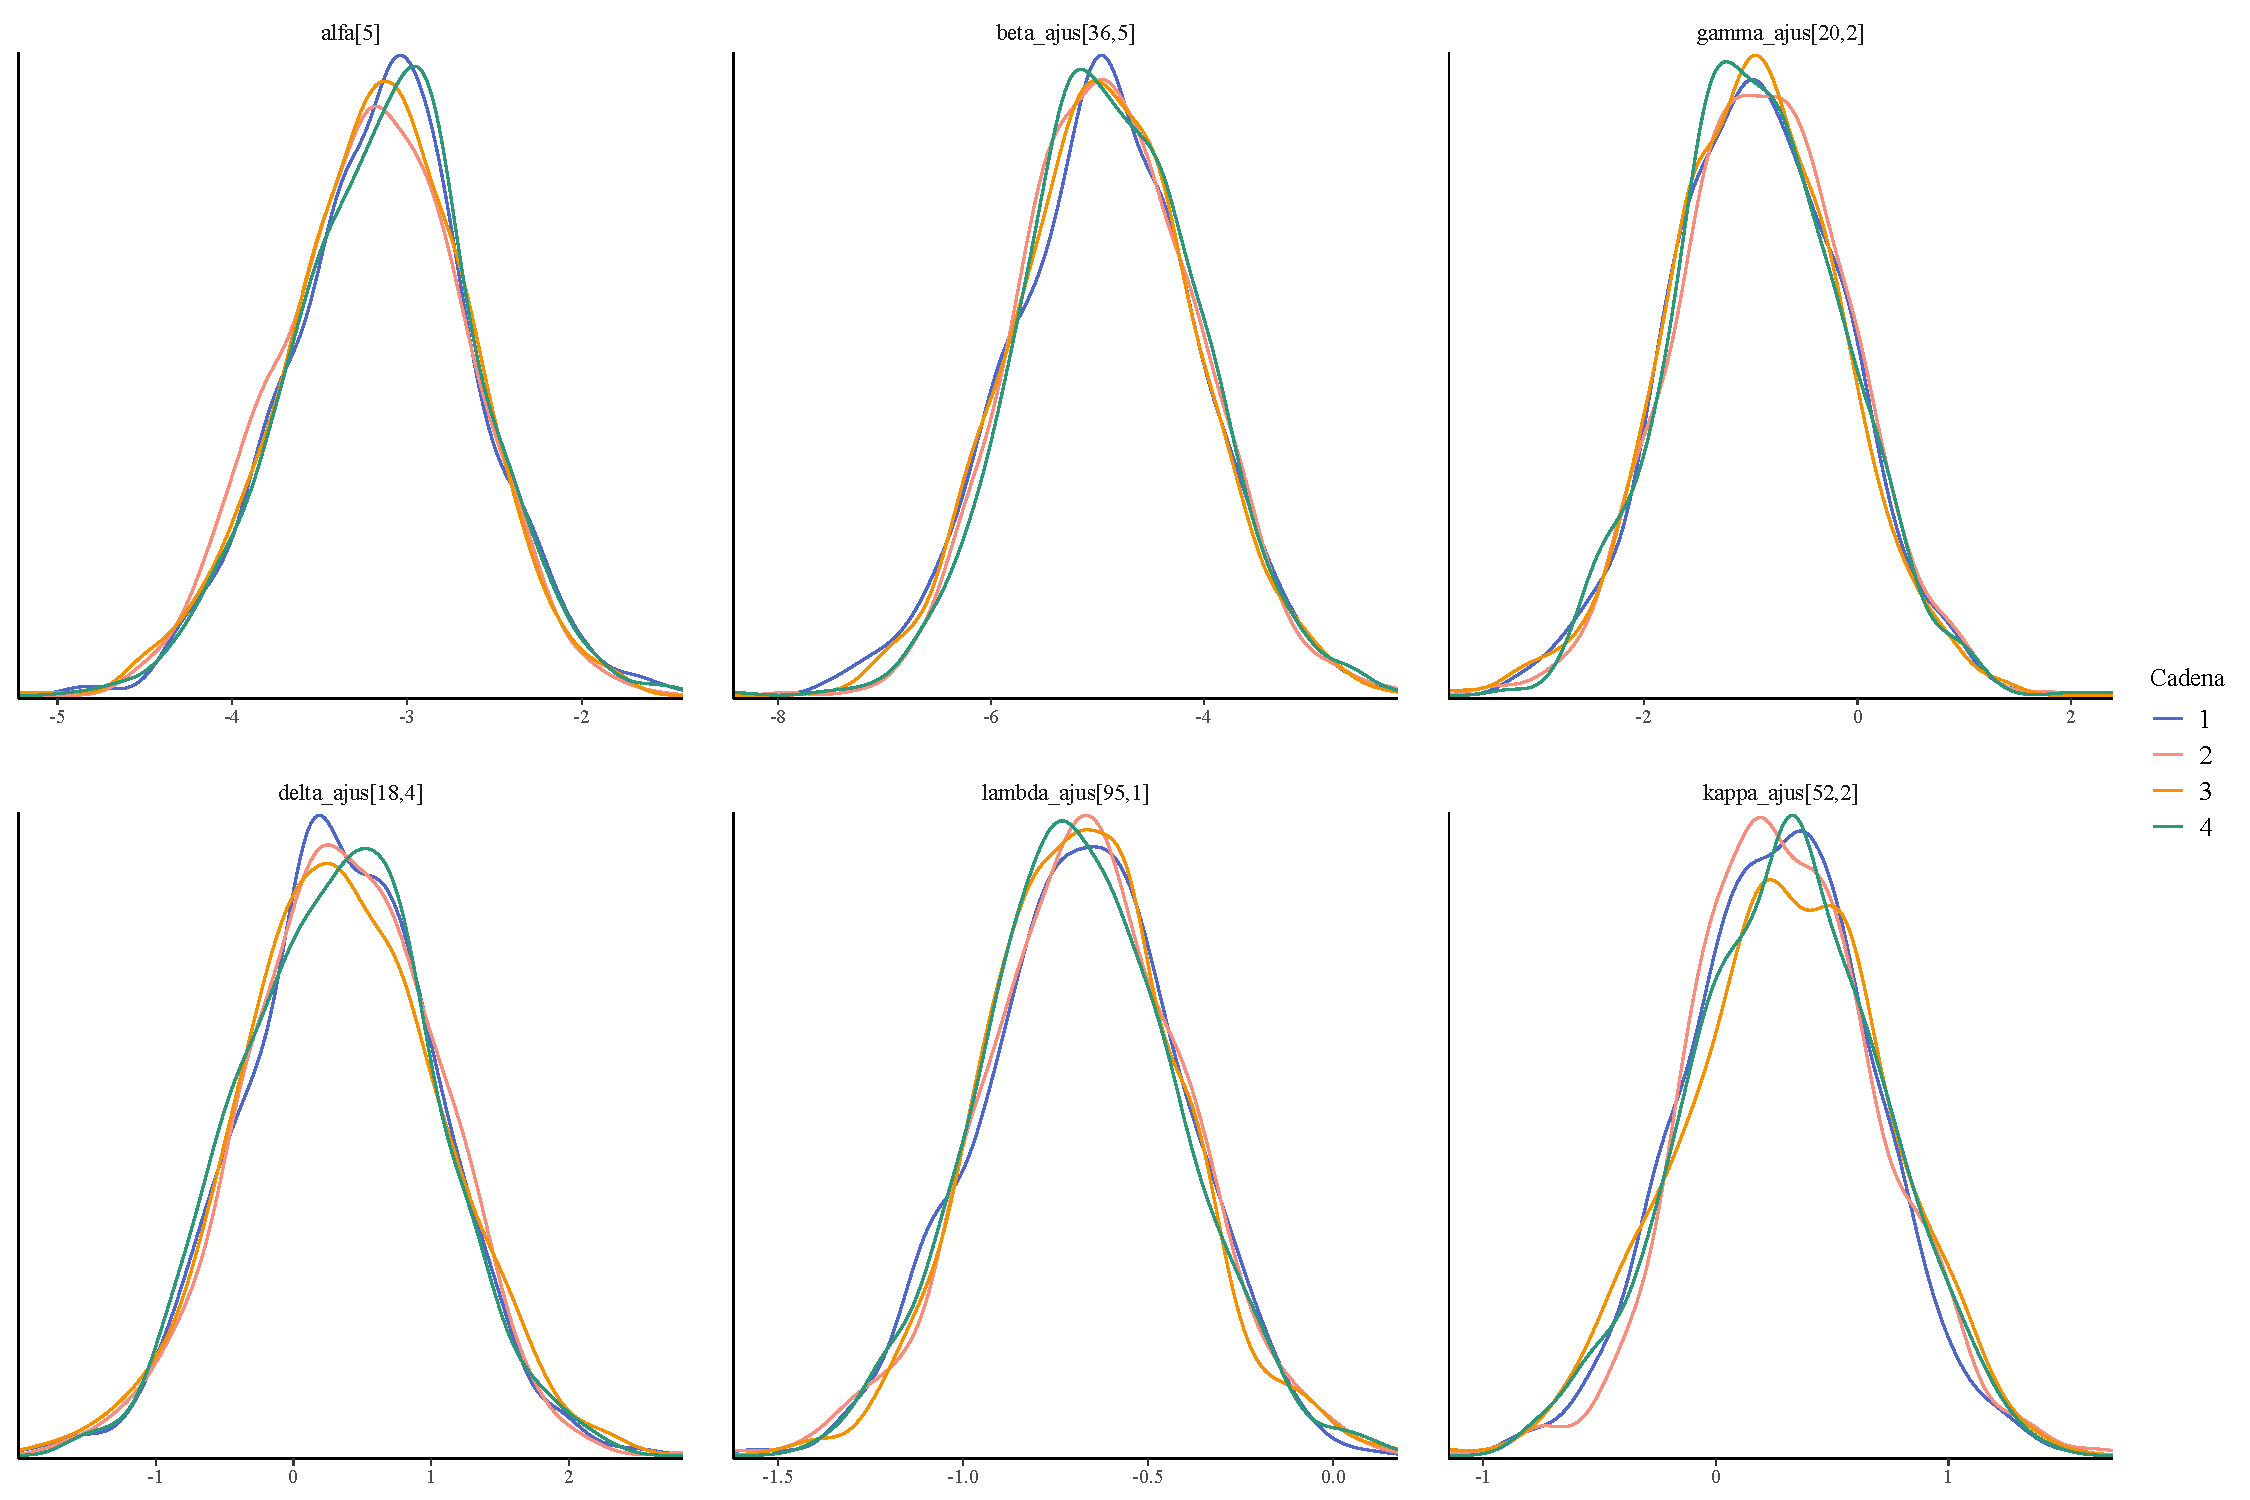
\includegraphics[width = \textwidth]{Figs/Convergencia/Convergencia_Densidades}
	\caption{Ejemplo de gráficos de densidades por cadena para algunos parámetros del modelo H.}
	\label{fig:Densidades_H}
	\end{subfigure}
	~
	\begin{subfigure}{0.6\textwidth}
	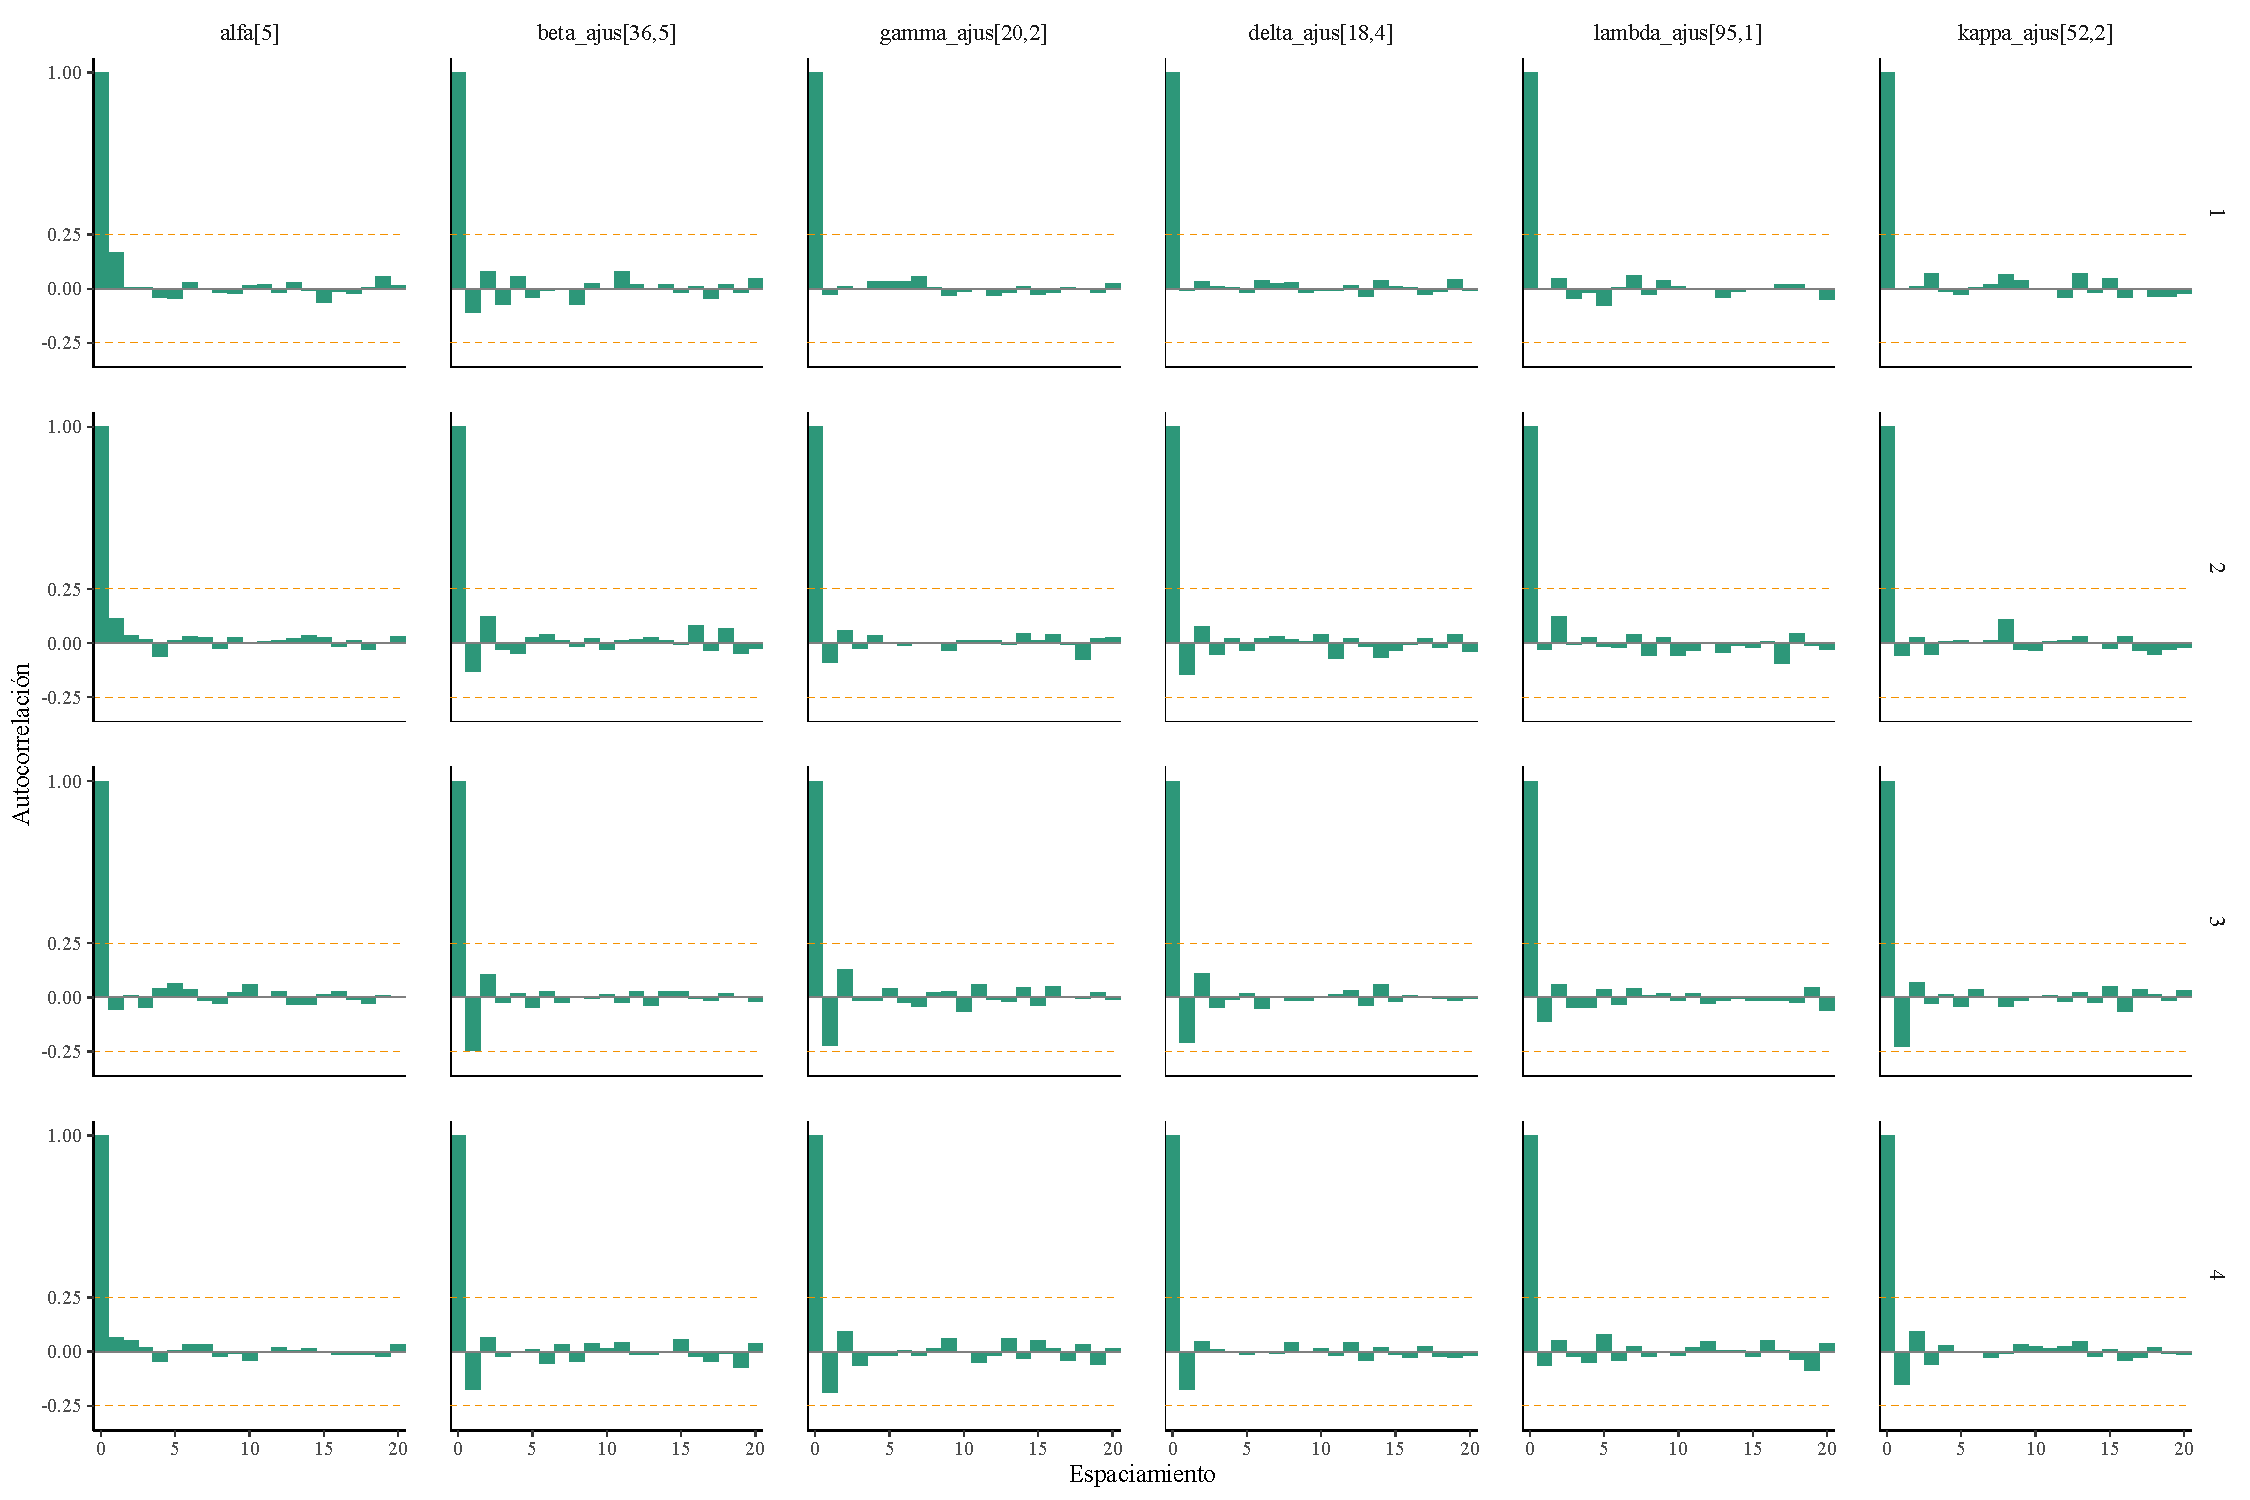
\includegraphics[width = \textwidth]{Figs/Convergencia/Convergencia_AutoCorr}
	\caption{Ejemplo de gráficos de autocorrelación para algunos parámetros del modelo H.}
	\label{fig:Autocorr_H}
	\end{subfigure}
	\caption{Fuente: elaboración propia.}
\end{figure}

 También analicé la convergencia del modelo H mediante los diagnósticos del paquete de $\mathsf{R}$ \textit{shinystan}, que permite de manera interactiva observar distintos gráficos y resúmenes respecto al ajuste del modelo vía HMC. De esta exploración, también concluí que el modelo satisfacía suficientemente bien la batería de diagnósticos para darnos confianza en que las muestras obtenidas provienen de la distribución posterior. Una vez verificada la convergencia, podemos proceder al análisis de los resultados para lo cual debemos interpretar lo que los coeficientes simulados nos dicen. 
 
\subsection{Definiendo efectos}

Interpretar los coeficientes de regresiones logísticas no es sencillo, pues estos se encuentran en una escala distinta a la de las proporciones o probabilidades que la liga logística define y que es en la que normalmente estamos interesados. Como explican \textcite{GelmanHill06}, además de las interpretaciones en términos de momios, un primer impulso a la hora de interpretar coeficientes es considerar el caso cuando la variable explicativa vale 1. Sin embargo, esto no siempre tiene sentido dependiendo del contexto en el que se realiza la regresión. Este es mi caso, por lo que no podría interpretar los coeficientes mediante alguna estrategia de ese tipo, sobre todo para evitar alguna falacia ecológica--- ver página \pageref{No_Extrapolar}---.\\ 

 Por ello, resultan útiles lo que los mismos autores llaman \textit{predictive comparisons}. Básicamente estos consisten en pensar en los efectos de los coeficientes en términos de una comparación entre dos valores distintos pero informativos de las variables explicativas de interés. Una alternativa de valores son la media y una desviación estándar por encima de ella. Esta elección tiene la ventaja de que, usualmente, se estaría realizando la interpretación en el rango de valores observado en la variable explicativa y no mediante una extrapolación. Hay que decir, no obstante, que una situación donde esto no sucede es cuando la variable explicativa observada es multimodal y la media cae en uno de los valles. Esta discusión general sobre alternativas de interpretación para regresiones logísticas puede consultarse en la referencia antes citada.\\ 
 
 Por nuestra parte, para fijar ideas, recordemos que las variables explicativas son las \textit{configuraciones sociales} definidas por las categorías poblacionales de las variables censales. Supongamos por ahora que estamos analizando un modelo individual nacional para una variable con 3 categorías, $x = (x_1,x_2,x_3)$. Recordando \eqref{eq:Modelo_Nal_Ind} y omitiendo el subíndice de las comunas, tendríamos que para alguna comuna en particular,

\begin{equation*}
ln\left(\dfrac{p}{1-p}\right) = \alpha + \beta_1 x_1 + \beta_2 x_2 + \beta_3 x_3.
\end{equation*}

Abusando de la notación, introduzco ahora unas expresiones. En primer lugar

\begin{equation*}
\eta(x;\beta_i)= \alpha + \beta_i x_i + \sum\limits_{k\neq i} \beta_k x_k, 
\end{equation*} 

para referirme al predictor lineal como función de la configuración social $x$ y considerando el intercepto $\alpha$ y los coeficientes como fijos. Sin embargo, ponemos énfasis en el coeficiente $\beta_i$ porque es el efecto que queremos interpretar. Asimismo tomemos 

\begin{equation*}
p(x;\beta_i)=\dfrac{e^{\eta(x;\beta_i)}}{1+e^{\eta(x;\beta_i)}}=\dfrac{1}{1+e^{-\eta(x;\beta_i)}}
\end{equation*} 

como el valor de la afinidad por Marine Le Pen en la comuna como función de la configuración social y, de nuevo, con el resto del predictor lineal fijo.\\

 Buscaríamos entonces definir el efecto que tiene el coeficiente $\beta_i$ como el cambio en puntos porcentuales para dicha afinidad cuando se pasa de una configuración a otra. Por ejemplo, suponiendo $x_{(0)}$ como una configuración inicial y $x_{(1)}$ como otra configuración en la que aumenta la categoría de interés, tendríamos que el efecto sería

\begin{equation*}
\Delta(\beta_i;x_{(0)},x_{(1)}) = p(x_{(1)};\beta_i)-p(x_{(0)};\beta_i)
\end{equation*}

Sin embargo, en nuestro caso no tenemos total libertad para elegir los valores $x_{(0)}$ y $x_{(1)}$ pues recordemos que son proporciones que deben sumar a 1. ¿Cómo elegirlos entonces?\\ 

En primer lugar, podemos seleccionar el punto de referencia $x_{(0)}$ como la media muestral, $x_{(0)}=\bar{x}=(\bar{x}_1,\bar{x}_2,\bar{x}_3)$. Posteriormente, como estamos interesados en el efecto del coeficiente $\beta_i$, empecemos a construir $x_{(1)}$ con base en $x_{(1),i}=\bar{x}_i + s_i$ donde $s_i$ es la desviación estándar muestral en la $i$-ésima categoría. Al agregarle una desviación estándar a $x_i$, para cumplir con la restricción, debemos disminuir su valor del resto de $x_k$s en su conjunto. Sin que sea la única forma de hacerlo, una propuesta es quitarle de manera proporcional a cada categoría restante una parte de la desviación estándar que sumamos a la categoría de interés. Esto sería de la siguiente manera: 

\begin{equation*}
x_{(1),k}=\bar{x}_k - s_i \dfrac{\bar{x}_k}{1-\bar{x}_i} \quad \forall k \neq i
\end{equation*}

Con este criterio podemos abusar un poco más de la notación. Si en lugar del caso específico de una configuración social de 3 categorías tenemos $l$ categorías, el efecto sería 

\begin{align}\label{eq:Efecto_Enchufado}
\Delta(\beta_i) &= p(x^\star;\beta_i)-p(\bar{x};\beta_i) \quad \forall i \in \mathbb{N}_l \\
\text{donde} \quad \bar{x} &= (\bar{x}_1,\dots,\bar{x}_{l}), \nonumber \\ 
x_i^\star = \bar{x}_i + s_i \quad &\text{y} \quad x_j^\star =\bar{x}_j - s_i\dfrac{\bar{x}_j}{1- \bar{x}_i} \quad \forall j \neq i\nonumber 
\end{align}

Ahora pensemos que querríamos calcular efectos para modelos jerárquicos. En este caso, simplemente reemplazamos el parámetro de interés por su equivalente jerárquico $\beta_{d,i}$ y tendríamos que calcular la media y la desviación estándar correspondiente dentro de cada departamento $d$: $\bar{x}_{d}$ y $s_{d,i}$. Esto lo indicamos mediante los subíndices:

\begin{equation}
\Delta(\beta_{d,i}) =  p(x^\star_{d};\beta_{d,i})-p(\bar{x}_{d};\beta_{d,i}) \quad \forall i \in \mathbb{N}_l
\end{equation}

¿Pero qué pasa cuando tenemos más de una variable? En esta situación, la decisión que tomé fue buscar una comparación \textit{c\ae teris paribus} en la que los sumandos del resto de variables explicativas del predictor lineal toman sus valores promedio en el departamento. Podemos también pensar que estamos modificando el intercepto con los sumandos del resto de categorías con valores promedio. Por ello, si asociamos a $x$ con la variable de la categoría de interés, $\beta$ con sus coeficientes y $z$ con el resto del predictor lineal, una notación más general podría ser

\begin{align}\label{eq:Efecto_Enchufado_Compuesto}
\Delta(\beta_{d,i};\bar{z}_d) &= p(x_d^\star;\beta_{d,i},\bar{z}_d)-p(\bar{x}_d;\beta_{d,i},\bar{z}_d) \quad \forall i \in \mathbb{N}_l \\
\text{donde} \quad p(x_d;\beta_{d,i},\bar{z}_d) &=\dfrac{1}{1+e^{-\eta(x_d;\beta_{d,i},\bar{z}_d)}} \nonumber \\
\text{y} \quad \eta(x_d;\beta_{d,i},\bar{z}_d) &= \bar{z}_d + \beta_{d,i}x_{d,i} + \sum\limits_{k\neq i} \beta_{d,k}x_{d,k}. \nonumber
\end{align}

Por ejemplo, en el caso del modelo compuesto A que incluye a la escolaridad y a las categorías socioprofesionales, el efecto para una categoría de escolaridad dependería del intercepto y las 8 categorías socioprofesionales vía $\bar{z}_d = \alpha_d + \sum\limits_{j=1}^8 \gamma_{d,k}\bar{x}_{csp,d,k}$.\\

Hasta aquí ya construimos una propuesta de efecto comparando dos predicciones específicas del modelo ``enchufando'' un valor específico o un estimador puntual de los coeficientes. Sin embargo, nuestro proceso de modelado bayesiano mediante HMC nos indica que tenemos incertidumbre sobre sus valores reflejada mediante muestras posteriores de valores simulados. Por lo mismo, siguiendo la única receta de la estadística bayesiana tendríamos que obtener la distribución posterior de los efectos, calculando \eqref{eq:Efecto_Enchufado_Compuesto} para cada simulación posterior $\beta_{d,i}^{(s)}$ y, correspondientemente, $\bar{z}_d^{(s)}$:

\begin{equation*}
\Delta(\beta_{d,i}^{(s)};\bar{z}_d^{(s)}) =  p(x^\star_{d};\beta_{d,i}^{(s)},\bar{z}_d^{(s)})-p(\bar{x}_{d};\beta_{d,i}^{(s)},\bar{z}_d^{(s)}) \quad \forall i \in \mathbb{N}_l ,\, s \in \mathbb{N}_S.
\end{equation*}

Esta sería la distribución posterior de los efectos con la que podemos continuar el análisis de los modelos mediante distintos resúmenes inferenciales como el efecto medio o mediano. También podríamos reportar intervalos centrales de probabilidad para al 95\%. Siguiendo la práctica común, cuando dichos intervalos contienen al 0, diríamos que la categoría poblacional no tiene un efecto significativo. Si, por el contrario, se encuentran en su totalidad por encima o por debajo del 0, diremos que se tiene un efecto positivo o negativo, respectivamente. 

\subsection{Efecto de la escolaridad}

